\documentclass[twoside]{book}

% Packages required by doxygen
\usepackage{calc}
\usepackage{doxygen}
\usepackage{graphicx}
\usepackage[utf8]{inputenc}
\usepackage{makeidx}
\usepackage{multicol}
\usepackage{multirow}
\usepackage{textcomp}
\usepackage[table]{xcolor}

% Font selection
\usepackage[T1]{fontenc}
\usepackage{mathptmx}
\usepackage[scaled=.90]{helvet}
\usepackage{courier}
\usepackage{amssymb}
\usepackage{sectsty}
\renewcommand{\familydefault}{\sfdefault}
\allsectionsfont{%
  \fontseries{bc}\selectfont%
  \color{darkgray}%
}
\renewcommand{\DoxyLabelFont}{%
  \fontseries{bc}\selectfont%
  \color{darkgray}%
}

% Page & text layout
\usepackage{geometry}
\geometry{%
  a4paper,%
  top=2.5cm,%
  bottom=2.5cm,%
  left=2.5cm,%
  right=2.5cm%
}
\tolerance=750
\hfuzz=15pt
\hbadness=750
\setlength{\emergencystretch}{15pt}
\setlength{\parindent}{0cm}
\setlength{\parskip}{0.2cm}
\makeatletter
\renewcommand{\paragraph}{%
  \@startsection{paragraph}{4}{0ex}{-1.0ex}{1.0ex}{%
    \normalfont\normalsize\bfseries\SS@parafont%
  }%
}
\renewcommand{\subparagraph}{%
  \@startsection{subparagraph}{5}{0ex}{-1.0ex}{1.0ex}{%
    \normalfont\normalsize\bfseries\SS@subparafont%
  }%
}
\makeatother

% Headers & footers
\usepackage{fancyhdr}
\pagestyle{fancyplain}
\fancyhead[LE]{\fancyplain{}{\bfseries\thepage}}
\fancyhead[CE]{\fancyplain{}{}}
\fancyhead[RE]{\fancyplain{}{\bfseries\leftmark}}
\fancyhead[LO]{\fancyplain{}{\bfseries\rightmark}}
\fancyhead[CO]{\fancyplain{}{}}
\fancyhead[RO]{\fancyplain{}{\bfseries\thepage}}
\fancyfoot[LE]{\fancyplain{}{}}
\fancyfoot[CE]{\fancyplain{}{}}
\fancyfoot[RE]{\fancyplain{}{\bfseries\scriptsize Generated on Sun Mar 20 2016 15\-:56\-:27 for Pomiar czasu przeszukania listy jednokierunkowej by Doxygen }}
\fancyfoot[LO]{\fancyplain{}{\bfseries\scriptsize Generated on Sun Mar 20 2016 15\-:56\-:27 for Pomiar czasu przeszukania listy jednokierunkowej by Doxygen }}
\fancyfoot[CO]{\fancyplain{}{}}
\fancyfoot[RO]{\fancyplain{}{}}
\renewcommand{\footrulewidth}{0.4pt}
\renewcommand{\chaptermark}[1]{%
  \markboth{#1}{}%
}
\renewcommand{\sectionmark}[1]{%
  \markright{\thesection\ #1}%
}

% Indices & bibliography
\usepackage{natbib}
\usepackage[titles]{tocloft}
\setcounter{tocdepth}{3}
\setcounter{secnumdepth}{5}
\makeindex

% Hyperlinks (required, but should be loaded last)
\usepackage{ifpdf}
\ifpdf
  \usepackage[pdftex,pagebackref=true]{hyperref}
\else
  \usepackage[ps2pdf,pagebackref=true]{hyperref}
\fi
\hypersetup{%
  colorlinks=true,%
  linkcolor=blue,%
  citecolor=blue,%
  unicode%
}

% Custom commands
\newcommand{\clearemptydoublepage}{%
  \newpage{\pagestyle{empty}\cleardoublepage}%
}


%===== C O N T E N T S =====

\begin{document}

% Titlepage & ToC
\hypersetup{pageanchor=false}
\pagenumbering{roman}
\begin{titlepage}
\vspace*{7cm}
\begin{center}%
{\Large Pomiar czasu przeszukania listy jednokierunkowej }\\
\vspace*{1cm}
{\large Generated by Doxygen 1.8.6}\\
\vspace*{0.5cm}
{\small Sun Mar 20 2016 15:56:27}\\
\end{center}
\end{titlepage}
\clearemptydoublepage
\tableofcontents
\clearemptydoublepage
\pagenumbering{arabic}
\hypersetup{pageanchor=true}

%--- Begin generated contents ---
\chapter{Opis programu}
\label{index}\hypertarget{index}{}\begin{DoxyAuthor}{Author}
Kamil Kuczaj \href{mailto:218478@student.pwr.edu.pl}{\tt 218478@student.\-pwr.\-edu.\-pl}
\end{DoxyAuthor}
\hypertarget{index_intro_sec}{}\section{Wstep}\label{index_intro_sec}
Program zostal zbudowany modulowo. W folderze inc/ znajduja sie pliki naglowkowe. Folder src/ zawiera pliki zrodlowe. W glownym folderze zbudowany zostal Makefile. Pliki obiektowe sa budowane w folderze obj/ a nastepnie linkowane do glownego folderu (prj/). Testowano przy wykorzystaniu kompilatora g++ w wersji 4.\-8.\-4 na systemie Linux Ubuntu 14.\-04.\-04 opartego o jądro 4.\-2.\-0-\/30-\/generic.\hypertarget{index_Licencja}{}\section{Licencja}\label{index_Licencja}
Program udostepniam na licencji G\-P\-Lv3.\hypertarget{index_install_sec}{}\section{Instalacja}\label{index_install_sec}
Aby zbudowac i jednoczesnie odpalic program\-: \$ make

Aby pozbyc sie plikow z koncowka $\ast$$\sim$ lub zaczynajacych sie na \#$\ast$\-: \$ make order

Aby pozbyc sie programu wykonywalnego oraz plikow obiektowych\-: \$ make clean

Aby wyswietlic pomoc do pliku Makefile\-: \$ make help 
\chapter{Hierarchical Index}
\section{Class Hierarchy}
This inheritance list is sorted roughly, but not completely, alphabetically\-:\begin{DoxyCompactList}
\item \contentsline{section}{I\-Lista$<$ List\-Type $>$}{\pageref{class_i_lista}}{}
\item \contentsline{section}{I\-Lista$<$ Type $>$}{\pageref{class_i_lista}}{}
\begin{DoxyCompactList}
\item \contentsline{section}{Lista$<$ Type $>$}{\pageref{class_lista}}{}
\end{DoxyCompactList}
\item \contentsline{section}{I\-Pojemnik$<$ Type $>$}{\pageref{class_i_pojemnik}}{}
\item \contentsline{section}{I\-Runnable}{\pageref{class_i_runnable}}{}
\begin{DoxyCompactList}
\item \contentsline{section}{Kolejka}{\pageref{class_kolejka}}{}
\item \contentsline{section}{Tablica$<$ Type $>$}{\pageref{class_tablica}}{}
\end{DoxyCompactList}
\item \contentsline{section}{I\-Stoper}{\pageref{class_i_stoper}}{}
\begin{DoxyCompactList}
\item \contentsline{section}{Stoper}{\pageref{class_stoper}}{}
\end{DoxyCompactList}
\item \contentsline{section}{Node$<$ Node\-Type $>$}{\pageref{class_node}}{}
\item \contentsline{section}{Node$<$ Type $>$}{\pageref{class_node}}{}
\item \contentsline{section}{Sedzia}{\pageref{class_sedzia}}{}
\end{DoxyCompactList}

\chapter{Class Index}
\section{Class List}
Here are the classes, structs, unions and interfaces with brief descriptions\-:\begin{DoxyCompactList}
\item\contentsline{section}{\hyperlink{class_i_lista}{I\-Lista$<$ List\-Type $>$} \\*Interfejs dla pojemnika \hyperlink{class_lista}{Lista} }{\pageref{class_i_lista}}{}
\item\contentsline{section}{\hyperlink{class_i_pojemnik}{I\-Pojemnik$<$ Type $>$} \\*Interfejs dla każdego pojemnika }{\pageref{class_i_pojemnik}}{}
\item\contentsline{section}{\hyperlink{class_i_runnable}{I\-Runnable} \\*Interfejs dla biegacza }{\pageref{class_i_runnable}}{}
\item\contentsline{section}{\hyperlink{class_i_stoper}{I\-Stoper} \\*Interfejs dla stopera }{\pageref{class_i_stoper}}{}
\item\contentsline{section}{\hyperlink{class_kolejka}{Kolejka} }{\pageref{class_kolejka}}{}
\item\contentsline{section}{\hyperlink{class_lista}{Lista$<$ Type $>$} \\*Klasa \hyperlink{class_lista}{Lista}, w ktorej odbywa sie zapis dynamiczny elementow typu int }{\pageref{class_lista}}{}
\item\contentsline{section}{\hyperlink{class_node}{Node$<$ Node\-Type $>$} \\*Imlementacja wezlow dla listy }{\pageref{class_node}}{}
\item\contentsline{section}{\hyperlink{class_sedzia}{Sedzia} \\*Implementacja klasy \hyperlink{class_sedzia}{Sedzia} }{\pageref{class_sedzia}}{}
\item\contentsline{section}{\hyperlink{class_stoper}{Stoper} \\*Implementacja klasy \hyperlink{class_stoper}{Stoper} }{\pageref{class_stoper}}{}
\item\contentsline{section}{\hyperlink{class_tablica}{Tablica$<$ Type $>$} \\*Klasa \hyperlink{class_tablica}{Tablica}, w ktorej odbywa sie zapis dynamiczny elementow }{\pageref{class_tablica}}{}
\end{DoxyCompactList}

\chapter{File Index}
\section{File List}
Here is a list of all files with brief descriptions\-:\begin{DoxyCompactList}
\item\contentsline{section}{inc/\hyperlink{_i_lista_8h}{I\-Lista.\-h} \\*Plik zawiera interfejs dla pojemnika \hyperlink{class_lista}{Lista} oraz dla klasy Wezel }{\pageref{_i_lista_8h}}{}
\item\contentsline{section}{inc/\hyperlink{_i_pojemnik_8h}{I\-Pojemnik.\-h} \\*Plik zawiera interfejs dla pojemnika Stos, \hyperlink{class_kolejka}{Kolejka} oraz \hyperlink{class_tablica}{Tablica} }{\pageref{_i_pojemnik_8h}}{}
\item\contentsline{section}{inc/\hyperlink{_i_runnable_8h}{I\-Runnable.\-h} \\*Naglowek zawierajacy interfejs dla biegacza }{\pageref{_i_runnable_8h}}{}
\item\contentsline{section}{inc/\hyperlink{_i_stoper_8h}{I\-Stoper.\-h} \\*Naglowek zawierajacy interfejs dla stopera }{\pageref{_i_stoper_8h}}{}
\item\contentsline{section}{inc/\hyperlink{_kolejka_8h}{Kolejka.\-h} }{\pageref{_kolejka_8h}}{}
\item\contentsline{section}{inc/\hyperlink{_lista_8h}{Lista.\-h} \\*Implementacja jednokierunkowej listy }{\pageref{_lista_8h}}{}
\item\contentsline{section}{inc/\hyperlink{_sedzia_8h}{Sedzia.\-h} \\*Naglowek opisujacy implementacje Sedziego }{\pageref{_sedzia_8h}}{}
\item\contentsline{section}{inc/\hyperlink{_stoper_8h}{Stoper.\-h} \\*Implementacja interfejsu \hyperlink{class_i_stoper}{I\-Stoper} w klasie \hyperlink{class_stoper}{Stoper} }{\pageref{_stoper_8h}}{}
\item\contentsline{section}{inc/\hyperlink{_stos_8h}{Stos.\-h} }{\pageref{_stos_8h}}{}
\item\contentsline{section}{inc/\hyperlink{_tablica_8h}{Tablica.\-h} \\*Implementacja interfesju \hyperlink{class_i_runnable}{I\-Runnable} }{\pageref{_tablica_8h}}{}
\item\contentsline{section}{src/\hyperlink{_kolejka_8cpp}{Kolejka.\-cpp} }{\pageref{_kolejka_8cpp}}{}
\item\contentsline{section}{src/\hyperlink{_lista_8cpp}{Lista.\-cpp} }{\pageref{_lista_8cpp}}{}
\item\contentsline{section}{src/\hyperlink{main_8cpp}{main.\-cpp} }{\pageref{main_8cpp}}{}
\item\contentsline{section}{src/\hyperlink{_sedzia_8cpp}{Sedzia.\-cpp} }{\pageref{_sedzia_8cpp}}{}
\item\contentsline{section}{src/\hyperlink{_stoper_8cpp}{Stoper.\-cpp} }{\pageref{_stoper_8cpp}}{}
\item\contentsline{section}{src/\hyperlink{_stos_8cpp}{Stos.\-cpp} }{\pageref{_stos_8cpp}}{}
\item\contentsline{section}{src/\hyperlink{_tablica_8cpp}{Tablica.\-cpp} }{\pageref{_tablica_8cpp}}{}
\end{DoxyCompactList}

\chapter{Class Documentation}
\hypertarget{class_i_lista}{\section{I\-Lista$<$ List\-Type $>$ Class Template Reference}
\label{class_i_lista}\index{I\-Lista$<$ List\-Type $>$@{I\-Lista$<$ List\-Type $>$}}
}


Interfejs dla pojemnika \hyperlink{class_lista}{Lista}.  




{\ttfamily \#include $<$I\-Lista.\-h$>$}

\subsection*{Protected Member Functions}
\begin{DoxyCompactItemize}
\item 
virtual void \hyperlink{class_i_lista_a756c44e78597aca5c7442645cf1f3cd5}{add} (List\-Type item, \hyperlink{_i_lista_8h_a91ad9478d81a7aaf2593e8d9c3d06a14}{uint} index)=0
\begin{DoxyCompactList}\small\item\em Wstawia element w dowolnym miejscu listy. \end{DoxyCompactList}\item 
virtual bool \hyperlink{class_i_lista_afbfc2fddaeb3cffb76cf92bb4a25ea1e}{remove} (\hyperlink{_i_lista_8h_a91ad9478d81a7aaf2593e8d9c3d06a14}{uint} index)=0
\begin{DoxyCompactList}\small\item\em Usuwa element z dowolnego miejsca listy. \end{DoxyCompactList}\item 
virtual bool \hyperlink{class_i_lista_ad902b7932a4d28d6c6c86d59111c4bd0}{is\-Empty} ()=0
\begin{DoxyCompactList}\small\item\em Sprawdza czy lista jest pusta. \end{DoxyCompactList}\item 
virtual List\-Type \hyperlink{class_i_lista_a6cf7937df214e06927df32046e231d08}{get} (\hyperlink{_i_lista_8h_a91ad9478d81a7aaf2593e8d9c3d06a14}{uint} index)=0
\begin{DoxyCompactList}\small\item\em Zwraca element z dowolnego miejsca listy. \end{DoxyCompactList}\item 
virtual \hyperlink{_i_lista_8h_a91ad9478d81a7aaf2593e8d9c3d06a14}{uint} \hyperlink{class_i_lista_a82a9479c66bc41f61e186769fa59c04b}{size} ()=0
\begin{DoxyCompactList}\small\item\em Zwraca rozmiar listy. \end{DoxyCompactList}\end{DoxyCompactItemize}


\subsection{Detailed Description}
\subsubsection*{template$<$class List\-Type$>$class I\-Lista$<$ List\-Type $>$}

Interfejs dla pojemnika \hyperlink{class_lista}{Lista}. 

Abstrakcyjna klasa, ktora zostala utworzona na potrzeby A\-D\-T Abstract Data Types. 

\subsection{Member Function Documentation}
\hypertarget{class_i_lista_a756c44e78597aca5c7442645cf1f3cd5}{\index{I\-Lista@{I\-Lista}!add@{add}}
\index{add@{add}!ILista@{I\-Lista}}
\subsubsection[{add}]{\setlength{\rightskip}{0pt plus 5cm}template$<$class List\-Type$>$ virtual void {\bf I\-Lista}$<$ List\-Type $>$\-::add (
\begin{DoxyParamCaption}
\item[{List\-Type}]{item, }
\item[{{\bf uint}}]{index}
\end{DoxyParamCaption}
)\hspace{0.3cm}{\ttfamily [protected]}, {\ttfamily [pure virtual]}}}\label{class_i_lista_a756c44e78597aca5c7442645cf1f3cd5}


Wstawia element w dowolnym miejscu listy. 

Wstawia element typu Type w miejsce wskazywane przez zmienna index.


\begin{DoxyParams}[1]{Parameters}
\mbox{\tt in}  & {\em item} & Element wstawiany. \\
\hline
\mbox{\tt in}  & {\em index} & Miejsce, w ktore ma byc wstawiony element item. \\
\hline
\end{DoxyParams}


Implemented in \hyperlink{class_lista_a5016da5359009ca7e3421de513cb3999}{Lista$<$ Type $>$}.

\hypertarget{class_i_lista_a6cf7937df214e06927df32046e231d08}{\index{I\-Lista@{I\-Lista}!get@{get}}
\index{get@{get}!ILista@{I\-Lista}}
\subsubsection[{get}]{\setlength{\rightskip}{0pt plus 5cm}template$<$class List\-Type$>$ virtual List\-Type {\bf I\-Lista}$<$ List\-Type $>$\-::get (
\begin{DoxyParamCaption}
\item[{{\bf uint}}]{index}
\end{DoxyParamCaption}
)\hspace{0.3cm}{\ttfamily [protected]}, {\ttfamily [pure virtual]}}}\label{class_i_lista_a6cf7937df214e06927df32046e231d08}


Zwraca element z dowolnego miejsca listy. 

Zwraca element z miejsca wskazywanego przez zmienna index.

\begin{DoxyReturn}{Returns}
Zwraca element typu Type. 
\end{DoxyReturn}


Implemented in \hyperlink{class_lista_aee227de057432c07d4045506b350ee14}{Lista$<$ Type $>$}.

\hypertarget{class_i_lista_ad902b7932a4d28d6c6c86d59111c4bd0}{\index{I\-Lista@{I\-Lista}!is\-Empty@{is\-Empty}}
\index{is\-Empty@{is\-Empty}!ILista@{I\-Lista}}
\subsubsection[{is\-Empty}]{\setlength{\rightskip}{0pt plus 5cm}template$<$class List\-Type$>$ virtual bool {\bf I\-Lista}$<$ List\-Type $>$\-::is\-Empty (
\begin{DoxyParamCaption}
{}
\end{DoxyParamCaption}
)\hspace{0.3cm}{\ttfamily [protected]}, {\ttfamily [pure virtual]}}}\label{class_i_lista_ad902b7932a4d28d6c6c86d59111c4bd0}


Sprawdza czy lista jest pusta. 

Sprawdza czy w liscie sa jakies elementy.


\begin{DoxyRetVals}{Return values}
{\em true} & \hyperlink{class_lista}{Lista} jest pusta. \\
\hline
{\em false} & \hyperlink{class_lista}{Lista} nie jest pusta. \\
\hline
\end{DoxyRetVals}


Implemented in \hyperlink{class_lista_acbc1b67a23e04ed8a6fd1ca378872c7d}{Lista$<$ Type $>$}.

\hypertarget{class_i_lista_afbfc2fddaeb3cffb76cf92bb4a25ea1e}{\index{I\-Lista@{I\-Lista}!remove@{remove}}
\index{remove@{remove}!ILista@{I\-Lista}}
\subsubsection[{remove}]{\setlength{\rightskip}{0pt plus 5cm}template$<$class List\-Type$>$ virtual bool {\bf I\-Lista}$<$ List\-Type $>$\-::remove (
\begin{DoxyParamCaption}
\item[{{\bf uint}}]{index}
\end{DoxyParamCaption}
)\hspace{0.3cm}{\ttfamily [protected]}, {\ttfamily [pure virtual]}}}\label{class_i_lista_afbfc2fddaeb3cffb76cf92bb4a25ea1e}


Usuwa element z dowolnego miejsca listy. 

Usuwa element z miejsca wskazywanego przez zmienna index.

\begin{DoxyReturn}{Returns}
Zwraca element typu Type. 
\end{DoxyReturn}


Implemented in \hyperlink{class_lista_a0513f36b0f98c1793a015e955b7274cb}{Lista$<$ Type $>$}.

\hypertarget{class_i_lista_a82a9479c66bc41f61e186769fa59c04b}{\index{I\-Lista@{I\-Lista}!size@{size}}
\index{size@{size}!ILista@{I\-Lista}}
\subsubsection[{size}]{\setlength{\rightskip}{0pt plus 5cm}template$<$class List\-Type$>$ virtual {\bf uint} {\bf I\-Lista}$<$ List\-Type $>$\-::size (
\begin{DoxyParamCaption}
{}
\end{DoxyParamCaption}
)\hspace{0.3cm}{\ttfamily [protected]}, {\ttfamily [pure virtual]}}}\label{class_i_lista_a82a9479c66bc41f61e186769fa59c04b}


Zwraca rozmiar listy. 

Zwraca ilosc elementow w liscie.

\begin{DoxyReturn}{Returns}
Rozmiar listy. 
\end{DoxyReturn}


Implemented in \hyperlink{class_lista_aff0cca3c261459240d16dfc64d397e5d}{Lista$<$ Type $>$}.



The documentation for this class was generated from the following file\-:\begin{DoxyCompactItemize}
\item 
inc/\hyperlink{_i_lista_8h}{I\-Lista.\-h}\end{DoxyCompactItemize}

\hypertarget{class_i_pojemnik}{\section{I\-Pojemnik$<$ Type $>$ Class Template Reference}
\label{class_i_pojemnik}\index{I\-Pojemnik$<$ Type $>$@{I\-Pojemnik$<$ Type $>$}}
}


Interfejs dla każdego pojemnika.  




{\ttfamily \#include $<$I\-Pojemnik.\-h$>$}

\subsection*{Protected Member Functions}
\begin{DoxyCompactItemize}
\item 
virtual Type \hyperlink{class_i_pojemnik_af344e1b83a85b421d97d4beccaa30322}{add} (Type item, \hyperlink{_i_lista_8h_a91ad9478d81a7aaf2593e8d9c3d06a14}{uint} index)=0
\begin{DoxyCompactList}\small\item\em Dodaje element w okreslonym miejscu. \end{DoxyCompactList}\item 
virtual Type \hyperlink{class_i_pojemnik_a95392ac62ce9417322986f870dd96191}{push} (\hyperlink{_i_lista_8h_a91ad9478d81a7aaf2593e8d9c3d06a14}{uint} index)=0
\begin{DoxyCompactList}\small\item\em Usuwa element z okreslonego miejsca. \end{DoxyCompactList}\item 
virtual Type \hyperlink{class_i_pojemnik_a699a1e80c731e602e8418f37c4707b96}{pop} (\hyperlink{_i_lista_8h_a91ad9478d81a7aaf2593e8d9c3d06a14}{uint} index)=0
\begin{DoxyCompactList}\small\item\em Usuwa element z pojemnika. \end{DoxyCompactList}\item 
virtual bool \hyperlink{class_i_pojemnik_ab4b01fcf2b3efc085722443dc083e1dc}{empty} ()=0
\begin{DoxyCompactList}\small\item\em Sprawdza czy pojemnika jest pusty. \end{DoxyCompactList}\item 
virtual \hyperlink{_i_lista_8h_a91ad9478d81a7aaf2593e8d9c3d06a14}{uint} \hyperlink{class_i_pojemnik_aed43b8d3b8114ce213eb182e80e35627}{size} ()=0
\begin{DoxyCompactList}\small\item\em Zwraca aktualny rozmiar pojemnika. \end{DoxyCompactList}\end{DoxyCompactItemize}


\subsection{Detailed Description}
\subsubsection*{template$<$class Type$>$class I\-Pojemnik$<$ Type $>$}

Interfejs dla każdego pojemnika. 

Abstrakcyjna klasa, ktora zostala utworzona na potrzeby A\-D\-T Abstract Data Types. 

\subsection{Member Function Documentation}
\hypertarget{class_i_pojemnik_af344e1b83a85b421d97d4beccaa30322}{\index{I\-Pojemnik@{I\-Pojemnik}!add@{add}}
\index{add@{add}!IPojemnik@{I\-Pojemnik}}
\subsubsection[{add}]{\setlength{\rightskip}{0pt plus 5cm}template$<$class Type $>$ virtual Type {\bf I\-Pojemnik}$<$ Type $>$\-::add (
\begin{DoxyParamCaption}
\item[{Type}]{item, }
\item[{{\bf uint}}]{index}
\end{DoxyParamCaption}
)\hspace{0.3cm}{\ttfamily [protected]}, {\ttfamily [pure virtual]}}}\label{class_i_pojemnik_af344e1b83a85b421d97d4beccaa30322}


Dodaje element w okreslonym miejscu. 

Metoda czysto wirtualna. Dodaje element item w miejscu index pojemnika.


\begin{DoxyParams}[1]{Parameters}
\mbox{\tt in}  & {\em item} & Dana, ktora ma byc wlozona. \\
\hline
\mbox{\tt in}  & {\em index} & Indeks, w ktorym ma znalezc sie nowa dana. \\
\hline
\end{DoxyParams}
\hypertarget{class_i_pojemnik_ab4b01fcf2b3efc085722443dc083e1dc}{\index{I\-Pojemnik@{I\-Pojemnik}!empty@{empty}}
\index{empty@{empty}!IPojemnik@{I\-Pojemnik}}
\subsubsection[{empty}]{\setlength{\rightskip}{0pt plus 5cm}template$<$class Type $>$ virtual bool {\bf I\-Pojemnik}$<$ Type $>$\-::empty (
\begin{DoxyParamCaption}
{}
\end{DoxyParamCaption}
)\hspace{0.3cm}{\ttfamily [protected]}, {\ttfamily [pure virtual]}}}\label{class_i_pojemnik_ab4b01fcf2b3efc085722443dc083e1dc}


Sprawdza czy pojemnika jest pusty. 

Sprawdza czy znajduja sie jakies elementy w pojemniku. Metoda czysto wirtualna.


\begin{DoxyRetVals}{Return values}
{\em true} & Pojemnik pusty. \\
\hline
{\em false} & Pojemnik nie jest pusty. \\
\hline
\end{DoxyRetVals}
\hypertarget{class_i_pojemnik_a699a1e80c731e602e8418f37c4707b96}{\index{I\-Pojemnik@{I\-Pojemnik}!pop@{pop}}
\index{pop@{pop}!IPojemnik@{I\-Pojemnik}}
\subsubsection[{pop}]{\setlength{\rightskip}{0pt plus 5cm}template$<$class Type $>$ virtual Type {\bf I\-Pojemnik}$<$ Type $>$\-::pop (
\begin{DoxyParamCaption}
\item[{{\bf uint}}]{index}
\end{DoxyParamCaption}
)\hspace{0.3cm}{\ttfamily [protected]}, {\ttfamily [pure virtual]}}}\label{class_i_pojemnik_a699a1e80c731e602e8418f37c4707b96}


Usuwa element z pojemnika. 

Usuwa element z pojemnika i zwraca go uzytkownikowi. Metoda czysto wirtualna.

\begin{DoxyReturn}{Returns}
Usuniety element. 
\end{DoxyReturn}
\hypertarget{class_i_pojemnik_a95392ac62ce9417322986f870dd96191}{\index{I\-Pojemnik@{I\-Pojemnik}!push@{push}}
\index{push@{push}!IPojemnik@{I\-Pojemnik}}
\subsubsection[{push}]{\setlength{\rightskip}{0pt plus 5cm}template$<$class Type $>$ virtual Type {\bf I\-Pojemnik}$<$ Type $>$\-::push (
\begin{DoxyParamCaption}
\item[{{\bf uint}}]{index}
\end{DoxyParamCaption}
)\hspace{0.3cm}{\ttfamily [protected]}, {\ttfamily [pure virtual]}}}\label{class_i_pojemnik_a95392ac62ce9417322986f870dd96191}


Usuwa element z okreslonego miejsca. 

Usuwa i zwraca podany element znajdujacy sie w index-\/owym miejscu.


\begin{DoxyParams}[1]{Parameters}
\mbox{\tt in}  & {\em index} & Indeks,z ktorego ma zostac usunieta dana. \\
\hline
\end{DoxyParams}
\hypertarget{class_i_pojemnik_aed43b8d3b8114ce213eb182e80e35627}{\index{I\-Pojemnik@{I\-Pojemnik}!size@{size}}
\index{size@{size}!IPojemnik@{I\-Pojemnik}}
\subsubsection[{size}]{\setlength{\rightskip}{0pt plus 5cm}template$<$class Type $>$ virtual {\bf uint} {\bf I\-Pojemnik}$<$ Type $>$\-::size (
\begin{DoxyParamCaption}
{}
\end{DoxyParamCaption}
)\hspace{0.3cm}{\ttfamily [protected]}, {\ttfamily [pure virtual]}}}\label{class_i_pojemnik_aed43b8d3b8114ce213eb182e80e35627}


Zwraca aktualny rozmiar pojemnika. 

Zwraca wartosc, ktora reprezentuje obecna ilosc elementow w pojemniku. Metoda czysto wirtualna.

\begin{DoxyReturn}{Returns}
Ilosc elementow w pojemniku. 
\end{DoxyReturn}


The documentation for this class was generated from the following file\-:\begin{DoxyCompactItemize}
\item 
inc/\hyperlink{_i_pojemnik_8h}{I\-Pojemnik.\-h}\end{DoxyCompactItemize}

\hypertarget{class_i_runnable}{\section{I\-Runnable Class Reference}
\label{class_i_runnable}\index{I\-Runnable@{I\-Runnable}}
}


Interfejs dla biegacza.  




{\ttfamily \#include $<$I\-Runnable.\-h$>$}



Inheritance diagram for I\-Runnable\-:
\nopagebreak
\begin{figure}[H]
\begin{center}
\leavevmode
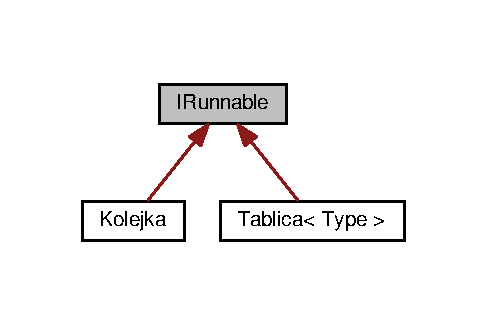
\includegraphics[width=234pt]{class_i_runnable__inherit__graph}
\end{center}
\end{figure}
\subsection*{Protected Member Functions}
\begin{DoxyCompactItemize}
\item 
virtual void \hyperlink{class_i_runnable_ac4d20dee4cb12c42eeed8698e839ddaf}{prepare} (unsigned int size)=0
\item 
virtual void \hyperlink{class_i_runnable_a6566fc2aa9fb5a7136f960172cee918d}{run} ()=0
\end{DoxyCompactItemize}


\subsection{Detailed Description}
Interfejs dla biegacza. 

Klasa abstrakcyjna z metodami czysto wirtualnymi. 

\subsection{Member Function Documentation}
\hypertarget{class_i_runnable_ac4d20dee4cb12c42eeed8698e839ddaf}{\index{I\-Runnable@{I\-Runnable}!prepare@{prepare}}
\index{prepare@{prepare}!IRunnable@{I\-Runnable}}
\subsubsection[{prepare}]{\setlength{\rightskip}{0pt plus 5cm}virtual void I\-Runnable\-::prepare (
\begin{DoxyParamCaption}
\item[{unsigned int}]{size}
\end{DoxyParamCaption}
)\hspace{0.3cm}{\ttfamily [protected]}, {\ttfamily [pure virtual]}}}\label{class_i_runnable_ac4d20dee4cb12c42eeed8698e839ddaf}


Implemented in \hyperlink{class_tablica_ac54e8c5dcbd665dcf48d10b9df8ff41b}{Tablica$<$ Type $>$}.

\hypertarget{class_i_runnable_a6566fc2aa9fb5a7136f960172cee918d}{\index{I\-Runnable@{I\-Runnable}!run@{run}}
\index{run@{run}!IRunnable@{I\-Runnable}}
\subsubsection[{run}]{\setlength{\rightskip}{0pt plus 5cm}virtual void I\-Runnable\-::run (
\begin{DoxyParamCaption}
{}
\end{DoxyParamCaption}
)\hspace{0.3cm}{\ttfamily [protected]}, {\ttfamily [pure virtual]}}}\label{class_i_runnable_a6566fc2aa9fb5a7136f960172cee918d}


Implemented in \hyperlink{class_tablica_a0e9570529b80cc6e1b40bf8b0d7e55c1}{Tablica$<$ Type $>$}.



The documentation for this class was generated from the following file\-:\begin{DoxyCompactItemize}
\item 
inc/\hyperlink{_i_runnable_8h}{I\-Runnable.\-h}\end{DoxyCompactItemize}

\hypertarget{class_i_stoper}{\section{I\-Stoper Class Reference}
\label{class_i_stoper}\index{I\-Stoper@{I\-Stoper}}
}


Interfejs dla stopera.  




{\ttfamily \#include $<$I\-Stoper.\-h$>$}



Inheritance diagram for I\-Stoper\-:
\nopagebreak
\begin{figure}[H]
\begin{center}
\leavevmode
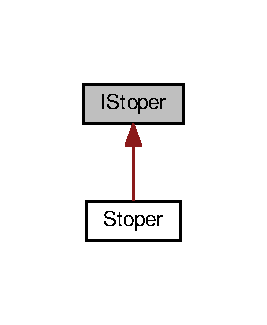
\includegraphics[width=128pt]{class_i_stoper__inherit__graph}
\end{center}
\end{figure}
\subsection*{Protected Member Functions}
\begin{DoxyCompactItemize}
\item 
virtual void \hyperlink{class_i_stoper_a17db649b3a90efc619022d35d6338f98}{start} ()=0
\item 
virtual void \hyperlink{class_i_stoper_acf2947911f2982372f21e8b0b1308520}{stop} ()=0
\item 
virtual double \hyperlink{class_i_stoper_abf0cb1128747e1a482ed487af6e6d114}{get\-Elapsed\-Time} ()=0
\item 
virtual void \hyperlink{class_i_stoper_ab0ce71cfe9db23e9b0016990816c1be2}{dump\-To\-File} (std\-::string file\-\_\-name)=0
\end{DoxyCompactItemize}


\subsection{Detailed Description}
Interfejs dla stopera. 

Klasa abstrakcyjna z metodami czysto wirtualnymi. 

\subsection{Member Function Documentation}
\hypertarget{class_i_stoper_ab0ce71cfe9db23e9b0016990816c1be2}{\index{I\-Stoper@{I\-Stoper}!dump\-To\-File@{dump\-To\-File}}
\index{dump\-To\-File@{dump\-To\-File}!IStoper@{I\-Stoper}}
\subsubsection[{dump\-To\-File}]{\setlength{\rightskip}{0pt plus 5cm}virtual void I\-Stoper\-::dump\-To\-File (
\begin{DoxyParamCaption}
\item[{std\-::string}]{file\-\_\-name}
\end{DoxyParamCaption}
)\hspace{0.3cm}{\ttfamily [protected]}, {\ttfamily [pure virtual]}}}\label{class_i_stoper_ab0ce71cfe9db23e9b0016990816c1be2}


Implemented in \hyperlink{class_stoper_a8896c3b2fa5428e29e5fef7f7bad3615}{Stoper}.

\hypertarget{class_i_stoper_abf0cb1128747e1a482ed487af6e6d114}{\index{I\-Stoper@{I\-Stoper}!get\-Elapsed\-Time@{get\-Elapsed\-Time}}
\index{get\-Elapsed\-Time@{get\-Elapsed\-Time}!IStoper@{I\-Stoper}}
\subsubsection[{get\-Elapsed\-Time}]{\setlength{\rightskip}{0pt plus 5cm}virtual double I\-Stoper\-::get\-Elapsed\-Time (
\begin{DoxyParamCaption}
{}
\end{DoxyParamCaption}
)\hspace{0.3cm}{\ttfamily [protected]}, {\ttfamily [pure virtual]}}}\label{class_i_stoper_abf0cb1128747e1a482ed487af6e6d114}


Implemented in \hyperlink{class_stoper_a8f50bbba9cb719ca9d573a5cb4a19e36}{Stoper}.

\hypertarget{class_i_stoper_a17db649b3a90efc619022d35d6338f98}{\index{I\-Stoper@{I\-Stoper}!start@{start}}
\index{start@{start}!IStoper@{I\-Stoper}}
\subsubsection[{start}]{\setlength{\rightskip}{0pt plus 5cm}virtual void I\-Stoper\-::start (
\begin{DoxyParamCaption}
{}
\end{DoxyParamCaption}
)\hspace{0.3cm}{\ttfamily [protected]}, {\ttfamily [pure virtual]}}}\label{class_i_stoper_a17db649b3a90efc619022d35d6338f98}


Implemented in \hyperlink{class_stoper_ae9dc93f4113f2d3afbe3b67166a7615d}{Stoper}.

\hypertarget{class_i_stoper_acf2947911f2982372f21e8b0b1308520}{\index{I\-Stoper@{I\-Stoper}!stop@{stop}}
\index{stop@{stop}!IStoper@{I\-Stoper}}
\subsubsection[{stop}]{\setlength{\rightskip}{0pt plus 5cm}virtual void I\-Stoper\-::stop (
\begin{DoxyParamCaption}
{}
\end{DoxyParamCaption}
)\hspace{0.3cm}{\ttfamily [protected]}, {\ttfamily [pure virtual]}}}\label{class_i_stoper_acf2947911f2982372f21e8b0b1308520}


Implemented in \hyperlink{class_stoper_afa91decbc99ba7509f1129f77c03b443}{Stoper}.



The documentation for this class was generated from the following file\-:\begin{DoxyCompactItemize}
\item 
inc/\hyperlink{_i_stoper_8h}{I\-Stoper.\-h}\end{DoxyCompactItemize}

\hypertarget{class_kolejka}{\section{Kolejka Class Reference}
\label{class_kolejka}\index{Kolejka@{Kolejka}}
}


{\ttfamily \#include $<$Kolejka.\-h$>$}



Inheritance diagram for Kolejka\-:
\nopagebreak
\begin{figure}[H]
\begin{center}
\leavevmode
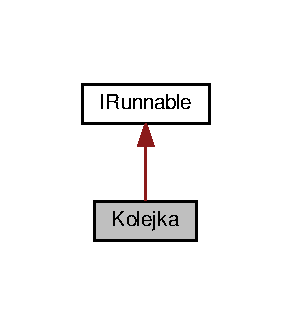
\includegraphics[width=140pt]{class_kolejka__inherit__graph}
\end{center}
\end{figure}


Collaboration diagram for Kolejka\-:
\nopagebreak
\begin{figure}[H]
\begin{center}
\leavevmode
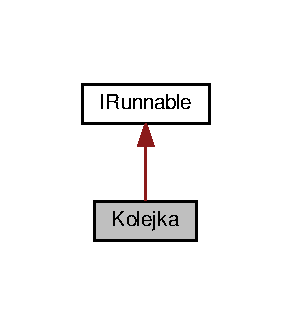
\includegraphics[width=140pt]{class_kolejka__coll__graph}
\end{center}
\end{figure}
\subsection*{Additional Inherited Members}


The documentation for this class was generated from the following file\-:\begin{DoxyCompactItemize}
\item 
inc/\hyperlink{_kolejka_8h}{Kolejka.\-h}\end{DoxyCompactItemize}

\hypertarget{class_lista}{\section{Lista$<$ Type $>$ Class Template Reference}
\label{class_lista}\index{Lista$<$ Type $>$@{Lista$<$ Type $>$}}
}


Klasa \hyperlink{class_lista}{Lista}, w ktorej odbywa sie zapis dynamiczny elementow typu int.  




{\ttfamily \#include $<$Lista.\-h$>$}



Inheritance diagram for Lista$<$ Type $>$\-:
\nopagebreak
\begin{figure}[H]
\begin{center}
\leavevmode
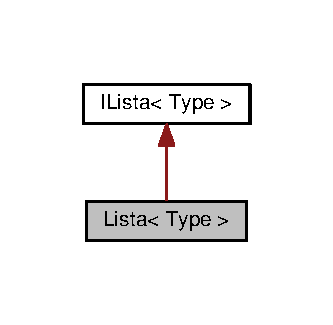
\includegraphics[width=160pt]{class_lista__inherit__graph}
\end{center}
\end{figure}


Collaboration diagram for Lista$<$ Type $>$\-:
\nopagebreak
\begin{figure}[H]
\begin{center}
\leavevmode
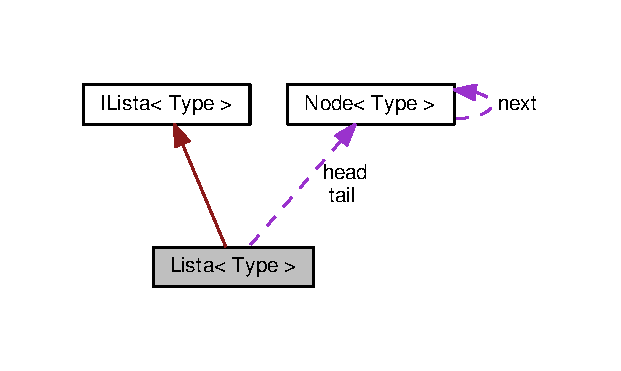
\includegraphics[width=298pt]{class_lista__coll__graph}
\end{center}
\end{figure}
\subsection*{Public Member Functions}
\begin{DoxyCompactItemize}
\item 
\hyperlink{class_lista_a9e74820e2d81e143c273992e563dffd3}{Lista} ()
\begin{DoxyCompactList}\small\item\em Konstruktor. \end{DoxyCompactList}\item 
\hyperlink{class_lista_a8de4b73bf5501c3fea7dd4041c320008}{$\sim$\-Lista} ()
\begin{DoxyCompactList}\small\item\em Destruktor. \end{DoxyCompactList}\item 
virtual void \hyperlink{class_lista_a5016da5359009ca7e3421de513cb3999}{add} (Type item, \hyperlink{_i_lista_8h_a91ad9478d81a7aaf2593e8d9c3d06a14}{uint} index)
\begin{DoxyCompactList}\small\item\em Wstawia element w dowolnym miejscu listy. \end{DoxyCompactList}\item 
virtual bool \hyperlink{class_lista_a0513f36b0f98c1793a015e955b7274cb}{remove} (\hyperlink{_i_lista_8h_a91ad9478d81a7aaf2593e8d9c3d06a14}{uint} index)
\begin{DoxyCompactList}\small\item\em Usuwa element z dowolnego miejsca listy. \end{DoxyCompactList}\item 
virtual bool \hyperlink{class_lista_acbc1b67a23e04ed8a6fd1ca378872c7d}{is\-Empty} ()
\begin{DoxyCompactList}\small\item\em Sprawdza czy lista jest pusta. \end{DoxyCompactList}\item 
virtual Type \hyperlink{class_lista_aee227de057432c07d4045506b350ee14}{get} (\hyperlink{_i_lista_8h_a91ad9478d81a7aaf2593e8d9c3d06a14}{uint} index)
\begin{DoxyCompactList}\small\item\em Zwraca element z dowolnego miejsca listy. \end{DoxyCompactList}\item 
virtual \hyperlink{_i_lista_8h_a91ad9478d81a7aaf2593e8d9c3d06a14}{uint} \hyperlink{class_lista_aff0cca3c261459240d16dfc64d397e5d}{size} ()
\begin{DoxyCompactList}\small\item\em Zwraca rozmiar listy. \end{DoxyCompactList}\item 
virtual \hyperlink{_i_lista_8h_a91ad9478d81a7aaf2593e8d9c3d06a14}{uint} \hyperlink{class_lista_a5b2885df007727df930fc293ef2ab2b2}{run} (Type desired\-\_\-element)
\begin{DoxyCompactList}\small\item\em Szuka elementu. \end{DoxyCompactList}\item 
virtual void \hyperlink{class_lista_a28b2f7513f4ec6596463f2b60f2a753b}{prepare} (\hyperlink{_i_lista_8h_a91ad9478d81a7aaf2593e8d9c3d06a14}{uint} desired\-\_\-size)
\begin{DoxyCompactList}\small\item\em Zapisuje liste slowami. \end{DoxyCompactList}\item 
void \hyperlink{class_lista_acfeb35d442b628fbcfb4db31e6acea16}{print} ()
\begin{DoxyCompactList}\small\item\em Wypisuje zawartosc listy. \end{DoxyCompactList}\end{DoxyCompactItemize}
\subsection*{Private Attributes}
\begin{DoxyCompactItemize}
\item 
\hyperlink{class_node}{Node}$<$ Type $>$ $\ast$ \hyperlink{class_lista_a9024fb7afb23ca1658288623fb940727}{head}
\begin{DoxyCompactList}\small\item\em Pierwszy element listy. \end{DoxyCompactList}\item 
\hyperlink{class_node}{Node}$<$ Type $>$ $\ast$ \hyperlink{class_lista_a510db6c07e6aa5802176451632f6bf4c}{tail}
\begin{DoxyCompactList}\small\item\em Ostatni element listy. \end{DoxyCompactList}\item 
\hyperlink{_i_lista_8h_a91ad9478d81a7aaf2593e8d9c3d06a14}{uint} \hyperlink{class_lista_a2ccdeaf5854898d0ba0fce725e0fa676}{size\-\_\-of\-\_\-list}
\begin{DoxyCompactList}\small\item\em Przechowuje rozmiar listy. \end{DoxyCompactList}\end{DoxyCompactItemize}
\subsection*{Additional Inherited Members}


\subsection{Detailed Description}
\subsubsection*{template$<$class Type$>$class Lista$<$ Type $>$}

Klasa \hyperlink{class_lista}{Lista}, w ktorej odbywa sie zapis dynamiczny elementow typu int. 

Implementuje metody interfejsu \hyperlink{class_i_runnable}{I\-Runnable}. Zajmuje sie dynamiczna alokacja pamieci. \hyperlink{class_lista}{Lista} jest dwukierunkowa oraz posiada mechanizm, dzieki ktoremu mamy dostep zarowno do pierwszego jak i ostatniego elementu. 

\subsection{Constructor \& Destructor Documentation}
\hypertarget{class_lista_a9e74820e2d81e143c273992e563dffd3}{\index{Lista@{Lista}!Lista@{Lista}}
\index{Lista@{Lista}!Lista@{Lista}}
\subsubsection[{Lista}]{\setlength{\rightskip}{0pt plus 5cm}template$<$class Type $>$ {\bf Lista}$<$ Type $>$\-::{\bf Lista} (
\begin{DoxyParamCaption}
{}
\end{DoxyParamCaption}
)}}\label{class_lista_a9e74820e2d81e143c273992e563dffd3}


Konstruktor. 

Tworzy poczatek listy. \hypertarget{class_lista_a8de4b73bf5501c3fea7dd4041c320008}{\index{Lista@{Lista}!$\sim$\-Lista@{$\sim$\-Lista}}
\index{$\sim$\-Lista@{$\sim$\-Lista}!Lista@{Lista}}
\subsubsection[{$\sim$\-Lista}]{\setlength{\rightskip}{0pt plus 5cm}template$<$class Type $>$ {\bf Lista}$<$ Type $>$\-::$\sim${\bf Lista} (
\begin{DoxyParamCaption}
{}
\end{DoxyParamCaption}
)}}\label{class_lista_a8de4b73bf5501c3fea7dd4041c320008}


Destruktor. 

Usuwa cala pamiec listy \char`\"{}skaczac\char`\"{} po jej elementach. 

\subsection{Member Function Documentation}
\hypertarget{class_lista_a5016da5359009ca7e3421de513cb3999}{\index{Lista@{Lista}!add@{add}}
\index{add@{add}!Lista@{Lista}}
\subsubsection[{add}]{\setlength{\rightskip}{0pt plus 5cm}template$<$class Type $>$ void {\bf Lista}$<$ Type $>$\-::add (
\begin{DoxyParamCaption}
\item[{Type}]{item, }
\item[{{\bf uint}}]{index}
\end{DoxyParamCaption}
)\hspace{0.3cm}{\ttfamily [virtual]}}}\label{class_lista_a5016da5359009ca7e3421de513cb3999}


Wstawia element w dowolnym miejscu listy. 

Wstawia element typu Type w miejsce wskazywane przez zmienna index.


\begin{DoxyParams}[1]{Parameters}
\mbox{\tt in}  & {\em item} & Element wstawiany. \\
\hline
\mbox{\tt in}  & {\em index} & Miejsce, w ktore ma byc wstawiony element item. \\
\hline
\end{DoxyParams}


Implements \hyperlink{class_i_lista_a756c44e78597aca5c7442645cf1f3cd5}{I\-Lista$<$ Type $>$}.

\hypertarget{class_lista_aee227de057432c07d4045506b350ee14}{\index{Lista@{Lista}!get@{get}}
\index{get@{get}!Lista@{Lista}}
\subsubsection[{get}]{\setlength{\rightskip}{0pt plus 5cm}template$<$class Type $>$ Type {\bf Lista}$<$ Type $>$\-::get (
\begin{DoxyParamCaption}
\item[{{\bf uint}}]{index}
\end{DoxyParamCaption}
)\hspace{0.3cm}{\ttfamily [virtual]}}}\label{class_lista_aee227de057432c07d4045506b350ee14}


Zwraca element z dowolnego miejsca listy. 

Zwraca element z miejsca wskazywanego przez zmienna index. Wyjatki są typu\-: const char $\ast$ \char`\"{}\-Empty list\char`\"{} -\/ pusta lista \char`\"{}\-Index out of bounds\char`\"{} -\/ przekroczono zakres, nie ma tylu elementow

\begin{DoxyReturn}{Returns}
Zwraca element typu Type. 
\end{DoxyReturn}


Implements \hyperlink{class_i_lista_a6cf7937df214e06927df32046e231d08}{I\-Lista$<$ Type $>$}.



Here is the caller graph for this function\-:
\nopagebreak
\begin{figure}[H]
\begin{center}
\leavevmode
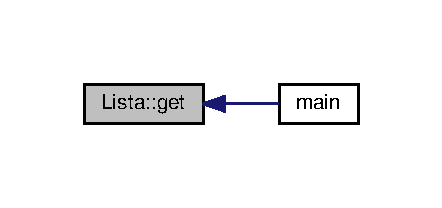
\includegraphics[width=212pt]{class_lista_aee227de057432c07d4045506b350ee14_icgraph}
\end{center}
\end{figure}


\hypertarget{class_lista_acbc1b67a23e04ed8a6fd1ca378872c7d}{\index{Lista@{Lista}!is\-Empty@{is\-Empty}}
\index{is\-Empty@{is\-Empty}!Lista@{Lista}}
\subsubsection[{is\-Empty}]{\setlength{\rightskip}{0pt plus 5cm}template$<$class Type $>$ bool {\bf Lista}$<$ Type $>$\-::is\-Empty (
\begin{DoxyParamCaption}
{}
\end{DoxyParamCaption}
)\hspace{0.3cm}{\ttfamily [virtual]}}}\label{class_lista_acbc1b67a23e04ed8a6fd1ca378872c7d}


Sprawdza czy lista jest pusta. 

Sprawdza czy w liscie sa jakies elementy.


\begin{DoxyRetVals}{Return values}
{\em true} & \hyperlink{class_lista}{Lista} jest pusta. \\
\hline
{\em false} & \hyperlink{class_lista}{Lista} nie jest pusta. \\
\hline
\end{DoxyRetVals}


Implements \hyperlink{class_i_lista_ad902b7932a4d28d6c6c86d59111c4bd0}{I\-Lista$<$ Type $>$}.

\hypertarget{class_lista_a28b2f7513f4ec6596463f2b60f2a753b}{\index{Lista@{Lista}!prepare@{prepare}}
\index{prepare@{prepare}!Lista@{Lista}}
\subsubsection[{prepare}]{\setlength{\rightskip}{0pt plus 5cm}template$<$class Type $>$ void {\bf Lista}$<$ Type $>$\-::prepare (
\begin{DoxyParamCaption}
\item[{{\bf uint}}]{desired\-\_\-size}
\end{DoxyParamCaption}
)\hspace{0.3cm}{\ttfamily [virtual]}}}\label{class_lista_a28b2f7513f4ec6596463f2b60f2a753b}


Zapisuje liste slowami. 

Zapisuje liste slowami zaczerpnietymi ze slownika. !!! W\-A\-Z\-N\-E !!!! Funkcja powinna byc uzyta tylko na poczatku, gdy cala lista jest pusta. Inaczej nastapi nadpisanie elementow poczatkowych.


\begin{DoxyParams}[1]{Parameters}
\mbox{\tt in}  & {\em desired\-\_\-size} & Ile elementow ma zostac wczytanych. \\
\hline
\end{DoxyParams}


Here is the caller graph for this function\-:
\nopagebreak
\begin{figure}[H]
\begin{center}
\leavevmode
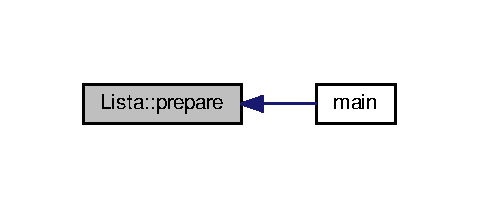
\includegraphics[width=230pt]{class_lista_a28b2f7513f4ec6596463f2b60f2a753b_icgraph}
\end{center}
\end{figure}


\hypertarget{class_lista_acfeb35d442b628fbcfb4db31e6acea16}{\index{Lista@{Lista}!print@{print}}
\index{print@{print}!Lista@{Lista}}
\subsubsection[{print}]{\setlength{\rightskip}{0pt plus 5cm}template$<$class Type $>$ void {\bf Lista}$<$ Type $>$\-::print (
\begin{DoxyParamCaption}
{}
\end{DoxyParamCaption}
)}}\label{class_lista_acfeb35d442b628fbcfb4db31e6acea16}


Wypisuje zawartosc listy. 

Wypisuje kazdy element listy w osobnej linii. Na gorze znajduje sie poczatek listy. 

Here is the caller graph for this function\-:
\nopagebreak
\begin{figure}[H]
\begin{center}
\leavevmode
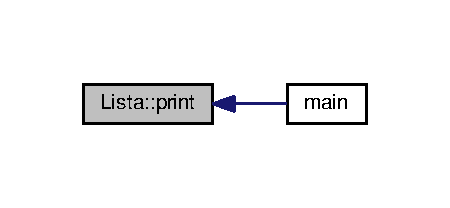
\includegraphics[width=216pt]{class_lista_acfeb35d442b628fbcfb4db31e6acea16_icgraph}
\end{center}
\end{figure}


\hypertarget{class_lista_a0513f36b0f98c1793a015e955b7274cb}{\index{Lista@{Lista}!remove@{remove}}
\index{remove@{remove}!Lista@{Lista}}
\subsubsection[{remove}]{\setlength{\rightskip}{0pt plus 5cm}template$<$class Type $>$ bool {\bf Lista}$<$ Type $>$\-::remove (
\begin{DoxyParamCaption}
\item[{{\bf uint}}]{index}
\end{DoxyParamCaption}
)\hspace{0.3cm}{\ttfamily [virtual]}}}\label{class_lista_a0513f36b0f98c1793a015e955b7274cb}


Usuwa element z dowolnego miejsca listy. 

Usuwa element z miejsca wskazywanego przez zmienna index.


\begin{DoxyRetVals}{Return values}
{\em true} & Udalo sie usunac element o podanym indeksie. \\
\hline
{\em false} & Nie udalo sie usunac elementu o podanym indeksie. \\
\hline
\end{DoxyRetVals}


Implements \hyperlink{class_i_lista_afbfc2fddaeb3cffb76cf92bb4a25ea1e}{I\-Lista$<$ Type $>$}.

\hypertarget{class_lista_a5b2885df007727df930fc293ef2ab2b2}{\index{Lista@{Lista}!run@{run}}
\index{run@{run}!Lista@{Lista}}
\subsubsection[{run}]{\setlength{\rightskip}{0pt plus 5cm}template$<$class Type $>$ {\bf uint} {\bf Lista}$<$ Type $>$\-::run (
\begin{DoxyParamCaption}
\item[{Type}]{desired\-\_\-element}
\end{DoxyParamCaption}
)\hspace{0.3cm}{\ttfamily [virtual]}}}\label{class_lista_a5b2885df007727df930fc293ef2ab2b2}


Szuka elementu. 

Szuka elementu wskazanego przez uzytkownika. W funkcji nastepuje Segmentation fault, gdy probujemy znalezc element, ktorego tam nie ma. W ogole sposob kodowania bledow gdy na nie napotka jest debilny ale nie mialem wystarczajaco duzo czasu aby to przerobic.


\begin{DoxyParams}[1]{Parameters}
\mbox{\tt in}  & {\em desired\-\_\-element} & Poszukiwana fraza.\\
\hline
\end{DoxyParams}

\begin{DoxyRetVals}{Return values}
{\em index$>$0} & Znalazl element i wyswietlil. \\
\hline
{\em 1199999999} & Nie znalazl i nie wyswietlil elementu. Wybrana wartosc, poniewaz nigdy tak duzej liczby elementow nie wczytamy. 10 cyfr. \\
\hline
{\em 1198989898} & \hyperlink{class_lista}{Lista} pusta. Wybrana wartosc, poniewaz nigdy tak duzej liczby elementow nie wczytamy. 10 cyfr. \\
\hline
\end{DoxyRetVals}
\hypertarget{class_lista_aff0cca3c261459240d16dfc64d397e5d}{\index{Lista@{Lista}!size@{size}}
\index{size@{size}!Lista@{Lista}}
\subsubsection[{size}]{\setlength{\rightskip}{0pt plus 5cm}template$<$class Type $>$ {\bf uint} {\bf Lista}$<$ Type $>$\-::size (
\begin{DoxyParamCaption}
{}
\end{DoxyParamCaption}
)\hspace{0.3cm}{\ttfamily [virtual]}}}\label{class_lista_aff0cca3c261459240d16dfc64d397e5d}


Zwraca rozmiar listy. 

Zwraca ilosc elementow w liscie.

\begin{DoxyReturn}{Returns}
Rozmiar listy. 
\end{DoxyReturn}


Implements \hyperlink{class_i_lista_a82a9479c66bc41f61e186769fa59c04b}{I\-Lista$<$ Type $>$}.



Here is the caller graph for this function\-:
\nopagebreak
\begin{figure}[H]
\begin{center}
\leavevmode
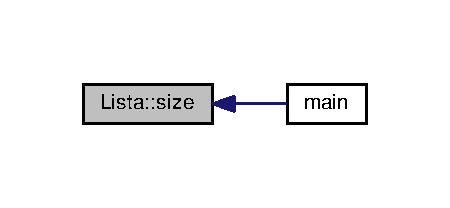
\includegraphics[width=216pt]{class_lista_aff0cca3c261459240d16dfc64d397e5d_icgraph}
\end{center}
\end{figure}




\subsection{Member Data Documentation}
\hypertarget{class_lista_a9024fb7afb23ca1658288623fb940727}{\index{Lista@{Lista}!head@{head}}
\index{head@{head}!Lista@{Lista}}
\subsubsection[{head}]{\setlength{\rightskip}{0pt plus 5cm}template$<$class Type$>$ {\bf Node}$<$Type$>$$\ast$ {\bf Lista}$<$ Type $>$\-::head\hspace{0.3cm}{\ttfamily [private]}}}\label{class_lista_a9024fb7afb23ca1658288623fb940727}


Pierwszy element listy. 

Wskazuje na pierwszy element listy. \hypertarget{class_lista_a2ccdeaf5854898d0ba0fce725e0fa676}{\index{Lista@{Lista}!size\-\_\-of\-\_\-list@{size\-\_\-of\-\_\-list}}
\index{size\-\_\-of\-\_\-list@{size\-\_\-of\-\_\-list}!Lista@{Lista}}
\subsubsection[{size\-\_\-of\-\_\-list}]{\setlength{\rightskip}{0pt plus 5cm}template$<$class Type$>$ {\bf uint} {\bf Lista}$<$ Type $>$\-::size\-\_\-of\-\_\-list\hspace{0.3cm}{\ttfamily [private]}}}\label{class_lista_a2ccdeaf5854898d0ba0fce725e0fa676}


Przechowuje rozmiar listy. 

Dzieki zastosowaniu tej zmiennej, o wiele latwiej poslugiwac sie lista. \hypertarget{class_lista_a510db6c07e6aa5802176451632f6bf4c}{\index{Lista@{Lista}!tail@{tail}}
\index{tail@{tail}!Lista@{Lista}}
\subsubsection[{tail}]{\setlength{\rightskip}{0pt plus 5cm}template$<$class Type$>$ {\bf Node}$<$Type$>$$\ast$ {\bf Lista}$<$ Type $>$\-::tail\hspace{0.3cm}{\ttfamily [private]}}}\label{class_lista_a510db6c07e6aa5802176451632f6bf4c}


Ostatni element listy. 

Wskazuje na ostatni element listy. 

The documentation for this class was generated from the following file\-:\begin{DoxyCompactItemize}
\item 
inc/\hyperlink{_lista_8h}{Lista.\-h}\end{DoxyCompactItemize}

\hypertarget{class_node}{\section{Node$<$ Node\-Type $>$ Class Template Reference}
\label{class_node}\index{Node$<$ Node\-Type $>$@{Node$<$ Node\-Type $>$}}
}


Imlementacja wezlow dla listy.  




{\ttfamily \#include $<$I\-Lista.\-h$>$}

\subsection*{Public Member Functions}
\begin{DoxyCompactItemize}
\item 
Node\-Type \hyperlink{class_node_a269284208819633cd6236f4da3c6bb68}{get\-Elem} ()
\begin{DoxyCompactList}\small\item\em Dostep do pola element. \end{DoxyCompactList}\item 
\hyperlink{class_node}{Node} \hyperlink{class_node_a4682a79b0e1b2ff33ce06fd0c8c5d6c7}{get\-Next} ()
\begin{DoxyCompactList}\small\item\em Dostep do nastepnego wezla. \end{DoxyCompactList}\item 
void \hyperlink{class_node_a61dd2669b5fc024125c60dd7fa1d8a42}{set\-Elem} (const Node\-Type t)
\begin{DoxyCompactList}\small\item\em Ustawia pole element. \end{DoxyCompactList}\item 
void \hyperlink{class_node_ae4c31b2f94885e6a4450a4f9f3d059af}{set\-Next} (\hyperlink{class_node}{Node}$<$ Node\-Type $>$ $\ast$t)
\begin{DoxyCompactList}\small\item\em Ustawia nastepny wezel. \end{DoxyCompactList}\end{DoxyCompactItemize}
\subsection*{Public Attributes}
\begin{DoxyCompactItemize}
\item 
Node\-Type \hyperlink{class_node_a7ae3a8a0cf4c0d490402599bd5d11c88}{element}
\begin{DoxyCompactList}\small\item\em Element w wezle. \end{DoxyCompactList}\item 
\hyperlink{class_node}{Node}$<$ Node\-Type $>$ $\ast$ \hyperlink{class_node_aa95538a7c96479172f550fefc6cc0074}{next}
\begin{DoxyCompactList}\small\item\em Wskaznik na nastepny wezel. \end{DoxyCompactList}\end{DoxyCompactItemize}
\subsection*{Friends}
\begin{DoxyCompactItemize}
\item 
{\footnotesize template$<$class List\-Type $>$ }\\class \hyperlink{class_node_acf8340255f3eca607a6c72f6d9a81dfb}{I\-Lista}
\begin{DoxyCompactList}\small\item\em Zaprzyjaznienie interfejsu \hyperlink{class_i_lista}{I\-Lista}. \end{DoxyCompactList}\end{DoxyCompactItemize}


\subsection{Detailed Description}
\subsubsection*{template$<$class Node\-Type$>$class Node$<$ Node\-Type $>$}

Imlementacja wezlow dla listy. 

Potrzebne do implementacji interfejsu listy. 

\subsection{Member Function Documentation}
\hypertarget{class_node_a269284208819633cd6236f4da3c6bb68}{\index{Node@{Node}!get\-Elem@{get\-Elem}}
\index{get\-Elem@{get\-Elem}!Node@{Node}}
\subsubsection[{get\-Elem}]{\setlength{\rightskip}{0pt plus 5cm}template$<$class Node\-Type$>$ Node\-Type {\bf Node}$<$ Node\-Type $>$\-::get\-Elem (
\begin{DoxyParamCaption}
{}
\end{DoxyParamCaption}
)\hspace{0.3cm}{\ttfamily [inline]}}}\label{class_node_a269284208819633cd6236f4da3c6bb68}


Dostep do pola element. 

Wymuszone poprzez hermetyzacje.

\begin{DoxyReturn}{Returns}
Zwraca element typu Type. 
\end{DoxyReturn}
\hypertarget{class_node_a4682a79b0e1b2ff33ce06fd0c8c5d6c7}{\index{Node@{Node}!get\-Next@{get\-Next}}
\index{get\-Next@{get\-Next}!Node@{Node}}
\subsubsection[{get\-Next}]{\setlength{\rightskip}{0pt plus 5cm}template$<$class Node\-Type$>$ {\bf Node} {\bf Node}$<$ Node\-Type $>$\-::get\-Next (
\begin{DoxyParamCaption}
{}
\end{DoxyParamCaption}
)\hspace{0.3cm}{\ttfamily [inline]}}}\label{class_node_a4682a79b0e1b2ff33ce06fd0c8c5d6c7}


Dostep do nastepnego wezla. 

Wymuszone poprzez hermetyzacje.

\begin{DoxyReturn}{Returns}
Zwraca element typu \hyperlink{class_node}{Node}. 
\end{DoxyReturn}
\hypertarget{class_node_a61dd2669b5fc024125c60dd7fa1d8a42}{\index{Node@{Node}!set\-Elem@{set\-Elem}}
\index{set\-Elem@{set\-Elem}!Node@{Node}}
\subsubsection[{set\-Elem}]{\setlength{\rightskip}{0pt plus 5cm}template$<$class Node\-Type$>$ void {\bf Node}$<$ Node\-Type $>$\-::set\-Elem (
\begin{DoxyParamCaption}
\item[{const Node\-Type}]{t}
\end{DoxyParamCaption}
)\hspace{0.3cm}{\ttfamily [inline]}}}\label{class_node_a61dd2669b5fc024125c60dd7fa1d8a42}


Ustawia pole element. 

Wymuszone poprzez hermetyzacje.


\begin{DoxyParams}[1]{Parameters}
\mbox{\tt in}  & {\em Wartosc,ktora} & ma zostac zapisana do pola element. \\
\hline
\end{DoxyParams}
\hypertarget{class_node_ae4c31b2f94885e6a4450a4f9f3d059af}{\index{Node@{Node}!set\-Next@{set\-Next}}
\index{set\-Next@{set\-Next}!Node@{Node}}
\subsubsection[{set\-Next}]{\setlength{\rightskip}{0pt plus 5cm}template$<$class Node\-Type$>$ void {\bf Node}$<$ Node\-Type $>$\-::set\-Next (
\begin{DoxyParamCaption}
\item[{{\bf Node}$<$ Node\-Type $>$ $\ast$}]{t}
\end{DoxyParamCaption}
)\hspace{0.3cm}{\ttfamily [inline]}}}\label{class_node_ae4c31b2f94885e6a4450a4f9f3d059af}


Ustawia nastepny wezel. 

Wymuszone poprzez hermetyzacje.


\begin{DoxyParams}[1]{Parameters}
\mbox{\tt in}  & {\em t} & Wezel, ktory ma zostac przypisany do pola next. \\
\hline
\end{DoxyParams}


\subsection{Friends And Related Function Documentation}
\hypertarget{class_node_acf8340255f3eca607a6c72f6d9a81dfb}{\index{Node@{Node}!I\-Lista@{I\-Lista}}
\index{I\-Lista@{I\-Lista}!Node@{Node}}
\subsubsection[{I\-Lista}]{\setlength{\rightskip}{0pt plus 5cm}template$<$class Node\-Type$>$ template$<$class List\-Type $>$ friend class {\bf I\-Lista}\hspace{0.3cm}{\ttfamily [friend]}}}\label{class_node_acf8340255f3eca607a6c72f6d9a81dfb}


Zaprzyjaznienie interfejsu \hyperlink{class_i_lista}{I\-Lista}. 

Umozliwia dostep do wezlow dla listy. 

\subsection{Member Data Documentation}
\hypertarget{class_node_a7ae3a8a0cf4c0d490402599bd5d11c88}{\index{Node@{Node}!element@{element}}
\index{element@{element}!Node@{Node}}
\subsubsection[{element}]{\setlength{\rightskip}{0pt plus 5cm}template$<$class Node\-Type$>$ Node\-Type {\bf Node}$<$ Node\-Type $>$\-::element}}\label{class_node_a7ae3a8a0cf4c0d490402599bd5d11c88}


Element w wezle. 

Co jest w wezle. \hypertarget{class_node_aa95538a7c96479172f550fefc6cc0074}{\index{Node@{Node}!next@{next}}
\index{next@{next}!Node@{Node}}
\subsubsection[{next}]{\setlength{\rightskip}{0pt plus 5cm}template$<$class Node\-Type$>$ {\bf Node}$<$Node\-Type$>$$\ast$ {\bf Node}$<$ Node\-Type $>$\-::next}}\label{class_node_aa95538a7c96479172f550fefc6cc0074}


Wskaznik na nastepny wezel. 

Wskazuje na nastepny wezel. 

The documentation for this class was generated from the following file\-:\begin{DoxyCompactItemize}
\item 
inc/\hyperlink{_i_lista_8h}{I\-Lista.\-h}\end{DoxyCompactItemize}

\hypertarget{class_sedzia}{\section{Sedzia Class Reference}
\label{class_sedzia}\index{Sedzia@{Sedzia}}
}


Implementacja klasy \hyperlink{class_sedzia}{Sedzia}.  




{\ttfamily \#include $<$Sedzia.\-h$>$}

\subsection*{Public Member Functions}
\begin{DoxyCompactItemize}
\item 
bool \hyperlink{class_sedzia_a7ff9a723a873b366f96028394f79d8a7}{set\-Off} (unsigned int how\-\_\-many)
\begin{DoxyCompactList}\small\item\em Funkcja, w ktorej odbywa sie bieg. \end{DoxyCompactList}\end{DoxyCompactItemize}


\subsection{Detailed Description}
Implementacja klasy \hyperlink{class_sedzia}{Sedzia}. 

\hyperlink{class_sedzia}{Sedzia} wykorzystuje elementy klasy \hyperlink{class_stoper}{Stoper} oraz klasy \hyperlink{class_tablica}{Tablica}. Mierzy czas wypelniania elemntow Tablicy. 

\subsection{Member Function Documentation}
\hypertarget{class_sedzia_a7ff9a723a873b366f96028394f79d8a7}{\index{Sedzia@{Sedzia}!set\-Off@{set\-Off}}
\index{set\-Off@{set\-Off}!Sedzia@{Sedzia}}
\subsubsection[{set\-Off}]{\setlength{\rightskip}{0pt plus 5cm}bool Sedzia\-::set\-Off (
\begin{DoxyParamCaption}
\item[{unsigned int}]{how\-\_\-many}
\end{DoxyParamCaption}
)}}\label{class_sedzia_a7ff9a723a873b366f96028394f79d8a7}


Funkcja, w ktorej odbywa sie bieg. 

Podczas wykonywania tej funkcji uruchamiany jest \hyperlink{class_stoper}{Stoper} oraz wypelniany jest element klasy Tablic\-A po uprzednim jej przygotowaniu.


\begin{DoxyParams}{Parameters}
{\em how\-\_\-many} & Informacja iloma elementami ma zostac wypelniona tablica. \\
\hline
\end{DoxyParams}


Here is the call graph for this function\-:
\nopagebreak
\begin{figure}[H]
\begin{center}
\leavevmode
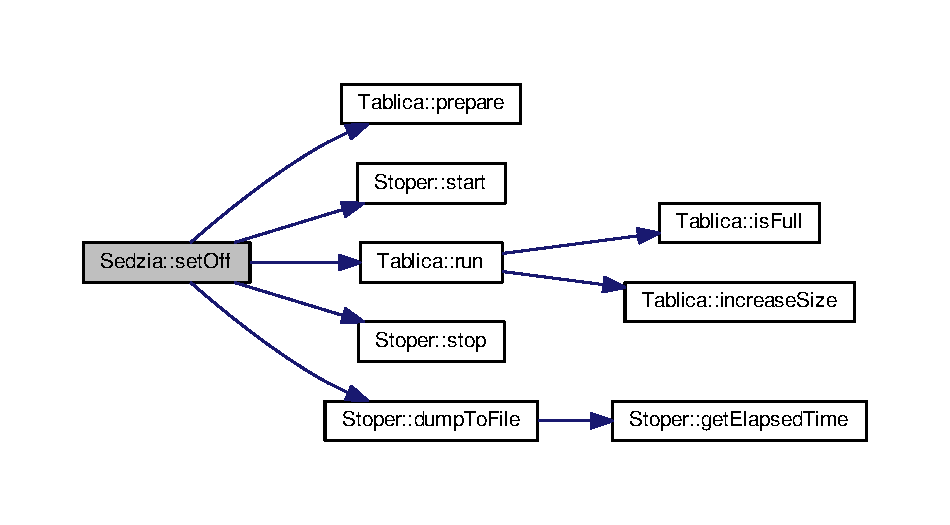
\includegraphics[width=350pt]{class_sedzia_a7ff9a723a873b366f96028394f79d8a7_cgraph}
\end{center}
\end{figure}




The documentation for this class was generated from the following files\-:\begin{DoxyCompactItemize}
\item 
inc/\hyperlink{_sedzia_8h}{Sedzia.\-h}\item 
src/\hyperlink{_sedzia_8cpp}{Sedzia.\-cpp}\end{DoxyCompactItemize}

\hypertarget{class_stoper}{\section{Stoper Class Reference}
\label{class_stoper}\index{Stoper@{Stoper}}
}


Implementacja klasy \hyperlink{class_stoper}{Stoper}.  




{\ttfamily \#include $<$Stoper.\-h$>$}



Inheritance diagram for Stoper\-:
\nopagebreak
\begin{figure}[H]
\begin{center}
\leavevmode
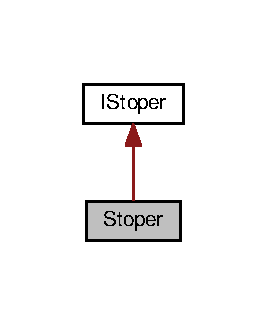
\includegraphics[width=128pt]{class_stoper__inherit__graph}
\end{center}
\end{figure}


Collaboration diagram for Stoper\-:
\nopagebreak
\begin{figure}[H]
\begin{center}
\leavevmode
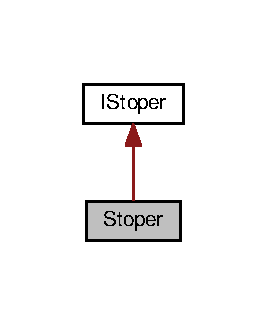
\includegraphics[width=128pt]{class_stoper__coll__graph}
\end{center}
\end{figure}
\subsection*{Public Member Functions}
\begin{DoxyCompactItemize}
\item 
virtual void \hyperlink{class_stoper_ae9dc93f4113f2d3afbe3b67166a7615d}{start} ()
\begin{DoxyCompactList}\small\item\em Implementacja funkcji \hyperlink{class_stoper_ae9dc93f4113f2d3afbe3b67166a7615d}{start()} z interfejsu \hyperlink{class_i_stoper}{I\-Stoper}. \end{DoxyCompactList}\item 
virtual void \hyperlink{class_stoper_afa91decbc99ba7509f1129f77c03b443}{stop} ()
\begin{DoxyCompactList}\small\item\em Implementacja funkcji \hyperlink{class_stoper_afa91decbc99ba7509f1129f77c03b443}{stop()} z interfejsu \hyperlink{class_i_stoper}{I\-Stoper}. \end{DoxyCompactList}\item 
virtual double \hyperlink{class_stoper_a8f50bbba9cb719ca9d573a5cb4a19e36}{get\-Elapsed\-Time} ()
\begin{DoxyCompactList}\small\item\em Implementacja funkcji get\-Elapse() z interfejsu \hyperlink{class_i_stoper}{I\-Stoper}. \end{DoxyCompactList}\item 
virtual void \hyperlink{class_stoper_a8896c3b2fa5428e29e5fef7f7bad3615}{dump\-To\-File} (std\-::string file\-\_\-name)
\begin{DoxyCompactList}\small\item\em Implementacja funkcji \hyperlink{class_stoper_a8896c3b2fa5428e29e5fef7f7bad3615}{dump\-To\-File()} z interfejsu \hyperlink{class_i_stoper}{I\-Stoper}. \end{DoxyCompactList}\end{DoxyCompactItemize}
\subsection*{Private Attributes}
\begin{DoxyCompactItemize}
\item 
clock\-\_\-t \hyperlink{class_stoper_a333b53d442ef20aa9ab907baf2c8f3b5}{start\-\_\-time}
\begin{DoxyCompactList}\small\item\em Moment startu stopera. \end{DoxyCompactList}\item 
clock\-\_\-t \hyperlink{class_stoper_a75fde898e50b0a40353881f51e7510d5}{stop\-\_\-time}
\begin{DoxyCompactList}\small\item\em Moment zatrzymania stopera. \end{DoxyCompactList}\item 
std\-::fstream \hyperlink{class_stoper_af4b77a51397bf1dfd324987685bc4d5b}{my\-\_\-file}
\begin{DoxyCompactList}\small\item\em Strumien zapisu do pliku. \end{DoxyCompactList}\end{DoxyCompactItemize}
\subsection*{Additional Inherited Members}


\subsection{Detailed Description}
Implementacja klasy \hyperlink{class_stoper}{Stoper}. 

W klasie \hyperlink{class_stoper}{Stoper} zostaly zaimplemetowane metody pozwalajace na pomiar czasu. Pomiar czasu odbywa sie dzieki bibliotece $<$ctime$>$ a zapis do pliku korzysta z biblioteki $<$fstream$>$. 

\subsection{Member Function Documentation}
\hypertarget{class_stoper_a8896c3b2fa5428e29e5fef7f7bad3615}{\index{Stoper@{Stoper}!dump\-To\-File@{dump\-To\-File}}
\index{dump\-To\-File@{dump\-To\-File}!Stoper@{Stoper}}
\subsubsection[{dump\-To\-File}]{\setlength{\rightskip}{0pt plus 5cm}void Stoper\-::dump\-To\-File (
\begin{DoxyParamCaption}
\item[{std\-::string}]{file\-\_\-name}
\end{DoxyParamCaption}
)\hspace{0.3cm}{\ttfamily [virtual]}}}\label{class_stoper_a8896c3b2fa5428e29e5fef7f7bad3615}


Implementacja funkcji \hyperlink{class_stoper_a8896c3b2fa5428e29e5fef7f7bad3615}{dump\-To\-File()} z interfejsu \hyperlink{class_i_stoper}{I\-Stoper}. 

Zapisuje zmierzony czas do pliku o nazwie \char`\"{}\$\{file\-\_\-name\}.\-csv\char`\"{}. Plik otwierany w trybie dopisywania (append) oraz wyjsciowym (out). Plik .csv to tzw. Comma-\/\-Separated Values -\/ latwo je potem zaimportowac do arkusza kalkulacyjnego oraz sa zgodne z ogolno przyjetym standardem.


\begin{DoxyParams}{Parameters}
{\em file\-\_\-name} & Nazwa pliku, do ktorego beda zapisane dane. Nazwa nie nie powinna zawierac rozszerzenia. Rozszerzenie jest dodawane w funkcji. \\
\hline
\end{DoxyParams}


Implements \hyperlink{class_i_stoper_ab0ce71cfe9db23e9b0016990816c1be2}{I\-Stoper}.



Here is the call graph for this function\-:
\nopagebreak
\begin{figure}[H]
\begin{center}
\leavevmode
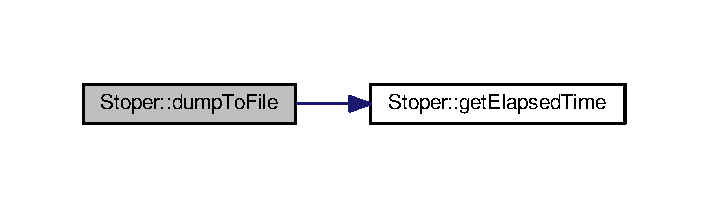
\includegraphics[width=340pt]{class_stoper_a8896c3b2fa5428e29e5fef7f7bad3615_cgraph}
\end{center}
\end{figure}




Here is the caller graph for this function\-:
\nopagebreak
\begin{figure}[H]
\begin{center}
\leavevmode
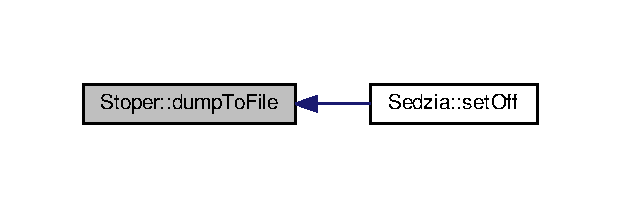
\includegraphics[width=298pt]{class_stoper_a8896c3b2fa5428e29e5fef7f7bad3615_icgraph}
\end{center}
\end{figure}


\hypertarget{class_stoper_a8f50bbba9cb719ca9d573a5cb4a19e36}{\index{Stoper@{Stoper}!get\-Elapsed\-Time@{get\-Elapsed\-Time}}
\index{get\-Elapsed\-Time@{get\-Elapsed\-Time}!Stoper@{Stoper}}
\subsubsection[{get\-Elapsed\-Time}]{\setlength{\rightskip}{0pt plus 5cm}double Stoper\-::get\-Elapsed\-Time (
\begin{DoxyParamCaption}
{}
\end{DoxyParamCaption}
)\hspace{0.3cm}{\ttfamily [virtual]}}}\label{class_stoper_a8f50bbba9cb719ca9d573a5cb4a19e36}


Implementacja funkcji get\-Elapse() z interfejsu \hyperlink{class_i_stoper}{I\-Stoper}. 

Oblicza czas pomiedzy czasem zapisanym w zmiennych start\-\_\-time i stop\-\_\-time.

\begin{DoxyReturn}{Returns}
Zwraca zmierzony czas -\/ roznica pomiedzy polem start\-\_\-time a polem stop\-\_\-time. 
\end{DoxyReturn}


Implements \hyperlink{class_i_stoper_abf0cb1128747e1a482ed487af6e6d114}{I\-Stoper}.



Here is the caller graph for this function\-:
\nopagebreak
\begin{figure}[H]
\begin{center}
\leavevmode
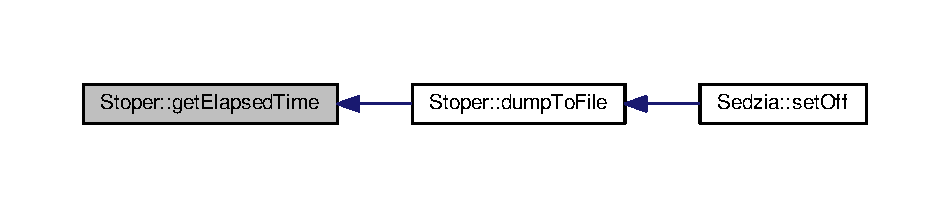
\includegraphics[width=350pt]{class_stoper_a8f50bbba9cb719ca9d573a5cb4a19e36_icgraph}
\end{center}
\end{figure}


\hypertarget{class_stoper_ae9dc93f4113f2d3afbe3b67166a7615d}{\index{Stoper@{Stoper}!start@{start}}
\index{start@{start}!Stoper@{Stoper}}
\subsubsection[{start}]{\setlength{\rightskip}{0pt plus 5cm}void Stoper\-::start (
\begin{DoxyParamCaption}
{}
\end{DoxyParamCaption}
)\hspace{0.3cm}{\ttfamily [virtual]}}}\label{class_stoper_ae9dc93f4113f2d3afbe3b67166a7615d}


Implementacja funkcji \hyperlink{class_stoper_ae9dc93f4113f2d3afbe3b67166a7615d}{start()} z interfejsu \hyperlink{class_i_stoper}{I\-Stoper}. 

Zapisuje moment uruchomienia stopera. 

Implements \hyperlink{class_i_stoper_a17db649b3a90efc619022d35d6338f98}{I\-Stoper}.



Here is the caller graph for this function\-:
\nopagebreak
\begin{figure}[H]
\begin{center}
\leavevmode
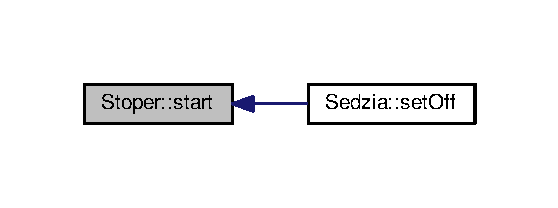
\includegraphics[width=268pt]{class_stoper_ae9dc93f4113f2d3afbe3b67166a7615d_icgraph}
\end{center}
\end{figure}


\hypertarget{class_stoper_afa91decbc99ba7509f1129f77c03b443}{\index{Stoper@{Stoper}!stop@{stop}}
\index{stop@{stop}!Stoper@{Stoper}}
\subsubsection[{stop}]{\setlength{\rightskip}{0pt plus 5cm}void Stoper\-::stop (
\begin{DoxyParamCaption}
{}
\end{DoxyParamCaption}
)\hspace{0.3cm}{\ttfamily [virtual]}}}\label{class_stoper_afa91decbc99ba7509f1129f77c03b443}


Implementacja funkcji \hyperlink{class_stoper_afa91decbc99ba7509f1129f77c03b443}{stop()} z interfejsu \hyperlink{class_i_stoper}{I\-Stoper}. 

Zapisuje moment zatrzymania stopera. 

Implements \hyperlink{class_i_stoper_acf2947911f2982372f21e8b0b1308520}{I\-Stoper}.



Here is the caller graph for this function\-:
\nopagebreak
\begin{figure}[H]
\begin{center}
\leavevmode
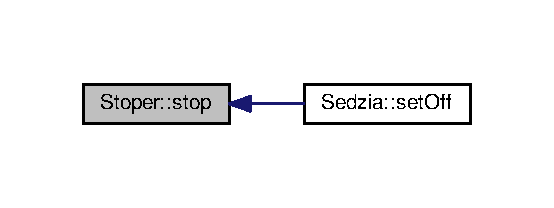
\includegraphics[width=266pt]{class_stoper_afa91decbc99ba7509f1129f77c03b443_icgraph}
\end{center}
\end{figure}




\subsection{Member Data Documentation}
\hypertarget{class_stoper_af4b77a51397bf1dfd324987685bc4d5b}{\index{Stoper@{Stoper}!my\-\_\-file@{my\-\_\-file}}
\index{my\-\_\-file@{my\-\_\-file}!Stoper@{Stoper}}
\subsubsection[{my\-\_\-file}]{\setlength{\rightskip}{0pt plus 5cm}std\-::fstream Stoper\-::my\-\_\-file\hspace{0.3cm}{\ttfamily [private]}}}\label{class_stoper_af4b77a51397bf1dfd324987685bc4d5b}


Strumien zapisu do pliku. 

Pole ulatwiajace zapis do pliku. \hypertarget{class_stoper_a333b53d442ef20aa9ab907baf2c8f3b5}{\index{Stoper@{Stoper}!start\-\_\-time@{start\-\_\-time}}
\index{start\-\_\-time@{start\-\_\-time}!Stoper@{Stoper}}
\subsubsection[{start\-\_\-time}]{\setlength{\rightskip}{0pt plus 5cm}clock\-\_\-t Stoper\-::start\-\_\-time\hspace{0.3cm}{\ttfamily [private]}}}\label{class_stoper_a333b53d442ef20aa9ab907baf2c8f3b5}


Moment startu stopera. 

Element przechowujacy informacje o czasie systemowym w momencie uruchomienia stopera. Element typu clock\-\_\-t. Nazwa zgodna konwencja podrecznika \char`\"{}\-Google C++ Style Guide\char`\"{}. \hypertarget{class_stoper_a75fde898e50b0a40353881f51e7510d5}{\index{Stoper@{Stoper}!stop\-\_\-time@{stop\-\_\-time}}
\index{stop\-\_\-time@{stop\-\_\-time}!Stoper@{Stoper}}
\subsubsection[{stop\-\_\-time}]{\setlength{\rightskip}{0pt plus 5cm}clock\-\_\-t Stoper\-::stop\-\_\-time\hspace{0.3cm}{\ttfamily [private]}}}\label{class_stoper_a75fde898e50b0a40353881f51e7510d5}


Moment zatrzymania stopera. 

Element przechowujacy informacje o czasie systemowym w momencie zatrzymania stopera. Element typu clock\-\_\-t. Nazwa zgodna konwencja podrecznika \char`\"{}\-Google C++ Style Guide\char`\"{}. 

The documentation for this class was generated from the following files\-:\begin{DoxyCompactItemize}
\item 
inc/\hyperlink{_stoper_8h}{Stoper.\-h}\item 
src/\hyperlink{_stoper_8cpp}{Stoper.\-cpp}\end{DoxyCompactItemize}

\hypertarget{class_tablica}{\section{Tablica$<$ Type $>$ Class Template Reference}
\label{class_tablica}\index{Tablica$<$ Type $>$@{Tablica$<$ Type $>$}}
}


Klasa \hyperlink{class_tablica}{Tablica}, w ktorej odbywa sie zapis dynamiczny elementow.  




{\ttfamily \#include $<$Tablica.\-h$>$}



Inheritance diagram for Tablica$<$ Type $>$\-:
\nopagebreak
\begin{figure}[H]
\begin{center}
\leavevmode
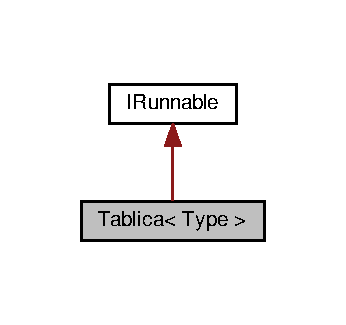
\includegraphics[width=166pt]{class_tablica__inherit__graph}
\end{center}
\end{figure}


Collaboration diagram for Tablica$<$ Type $>$\-:
\nopagebreak
\begin{figure}[H]
\begin{center}
\leavevmode
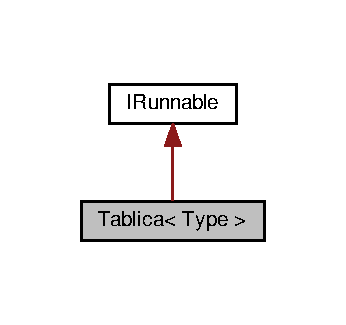
\includegraphics[width=166pt]{class_tablica__coll__graph}
\end{center}
\end{figure}
\subsection*{Public Member Functions}
\begin{DoxyCompactItemize}
\item 
\hyperlink{class_tablica_a3ebc24ff90be6556ec0c0fa87f354c81}{Tablica} (\hyperlink{_i_lista_8h_a91ad9478d81a7aaf2593e8d9c3d06a14}{uint} x=10)
\begin{DoxyCompactList}\small\item\em Konstruktor parametryczny. \end{DoxyCompactList}\item 
\hyperlink{class_tablica_aa41eb34f825167e33916793c807087ec}{$\sim$\-Tablica} ()
\begin{DoxyCompactList}\small\item\em Destruktor. \end{DoxyCompactList}\item 
virtual void \hyperlink{class_tablica_ac54e8c5dcbd665dcf48d10b9df8ff41b}{prepare} (\hyperlink{_i_lista_8h_a91ad9478d81a7aaf2593e8d9c3d06a14}{uint} size)
\begin{DoxyCompactList}\small\item\em Implementacja funkcji \hyperlink{class_tablica_ac54e8c5dcbd665dcf48d10b9df8ff41b}{prepare()} interfesju \hyperlink{class_i_runnable}{I\-Runnable}. \end{DoxyCompactList}\item 
virtual void \hyperlink{class_tablica_a0e9570529b80cc6e1b40bf8b0d7e55c1}{run} ()
\begin{DoxyCompactList}\small\item\em Implementacja funkcji \hyperlink{class_tablica_a0e9570529b80cc6e1b40bf8b0d7e55c1}{run()} interfesju \hyperlink{class_i_runnable}{I\-Runnable}. \end{DoxyCompactList}\item 
\hyperlink{_i_lista_8h_a91ad9478d81a7aaf2593e8d9c3d06a14}{uint} \hyperlink{class_tablica_ac3341812852356aa941c7077f7dfcfd7}{get\-Size} ()
\begin{DoxyCompactList}\small\item\em Zwraca aktualny rozmiar tablicy dynamicznej. \end{DoxyCompactList}\end{DoxyCompactItemize}
\subsection*{Private Member Functions}
\begin{DoxyCompactItemize}
\item 
bool \hyperlink{class_tablica_afbabf1c6a51051bd69c04e6c7306938c}{is\-Full} ()
\begin{DoxyCompactList}\small\item\em Pozwala prosto okreslic, czy nalezy przydzielic pamiec. \end{DoxyCompactList}\item 
void \hyperlink{class_tablica_a6c8a0a055eb2bda8e7e76cc5b7690652}{increase\-Size} ()
\begin{DoxyCompactList}\small\item\em Zwieksza rozmiar przydzielonej pamieci na stercie. \end{DoxyCompactList}\end{DoxyCompactItemize}
\subsection*{Private Attributes}
\begin{DoxyCompactItemize}
\item 
Type $\ast$ \hyperlink{class_tablica_a03f7862b518bdd503051388389949257}{elements}
\begin{DoxyCompactList}\small\item\em Wskaznik do poczatku tablicy dynamicznej. \end{DoxyCompactList}\item 
\hyperlink{_i_lista_8h_a91ad9478d81a7aaf2593e8d9c3d06a14}{uint} \hyperlink{class_tablica_aa2313b2db3dfda306acaf2a28be00707}{current\-\_\-size}
\begin{DoxyCompactList}\small\item\em Okresla aktualny rozmiar stosu. \end{DoxyCompactList}\item 
\hyperlink{_i_lista_8h_a91ad9478d81a7aaf2593e8d9c3d06a14}{uint} \hyperlink{class_tablica_ab9bd8738c20ec1d02ceff156af4675bc}{desired\-\_\-size}
\begin{DoxyCompactList}\small\item\em Okresla pozadany rozmiar stosu. \end{DoxyCompactList}\item 
unsigned int \hyperlink{class_tablica_ab05112ff73217668c456d7a92273574e}{index}
\begin{DoxyCompactList}\small\item\em Okresla aktualny indeks. \end{DoxyCompactList}\end{DoxyCompactItemize}


\subsection{Detailed Description}
\subsubsection*{template$<$class Type$>$class Tablica$<$ Type $>$}

Klasa \hyperlink{class_tablica}{Tablica}, w ktorej odbywa sie zapis dynamiczny elementow. 

Implementuje metody interfejsu \hyperlink{class_i_runnable}{I\-Runnable}. Zajmuje sie dynamiczna alokacja pamieci. Elastyczna a propos typow wskutek zastosowania szablonow. 

\subsection{Constructor \& Destructor Documentation}
\hypertarget{class_tablica_a3ebc24ff90be6556ec0c0fa87f354c81}{\index{Tablica@{Tablica}!Tablica@{Tablica}}
\index{Tablica@{Tablica}!Tablica@{Tablica}}
\subsubsection[{Tablica}]{\setlength{\rightskip}{0pt plus 5cm}template$<$class Type$>$ {\bf Tablica}$<$ Type $>$\-::{\bf Tablica} (
\begin{DoxyParamCaption}
\item[{{\bf uint}}]{x = {\ttfamily 10}}
\end{DoxyParamCaption}
)\hspace{0.3cm}{\ttfamily [inline]}}}\label{class_tablica_a3ebc24ff90be6556ec0c0fa87f354c81}


Konstruktor parametryczny. 

Umozliwia okreslenie poczatkowego rozmiaru tablicy. W przypadku braku okreslenia tego rozmiaru przyjmuje domyslna wartosc rowna 10.


\begin{DoxyParams}{Parameters}
{\em x} & Okresla poczatkowa wielkosc przydzielonej pamieci. Domyslna wartosc w przypadku braku podania to 10. \\
\hline
\end{DoxyParams}
\hypertarget{class_tablica_aa41eb34f825167e33916793c807087ec}{\index{Tablica@{Tablica}!$\sim$\-Tablica@{$\sim$\-Tablica}}
\index{$\sim$\-Tablica@{$\sim$\-Tablica}!Tablica@{Tablica}}
\subsubsection[{$\sim$\-Tablica}]{\setlength{\rightskip}{0pt plus 5cm}template$<$class Type$>$ {\bf Tablica}$<$ Type $>$\-::$\sim${\bf Tablica} (
\begin{DoxyParamCaption}
{}
\end{DoxyParamCaption}
)\hspace{0.3cm}{\ttfamily [inline]}}}\label{class_tablica_aa41eb34f825167e33916793c807087ec}


Destruktor. 

Usuwa pamiec przypisana komorce, na ktora wskazuje pole $\ast$elements. 

\subsection{Member Function Documentation}
\hypertarget{class_tablica_ac3341812852356aa941c7077f7dfcfd7}{\index{Tablica@{Tablica}!get\-Size@{get\-Size}}
\index{get\-Size@{get\-Size}!Tablica@{Tablica}}
\subsubsection[{get\-Size}]{\setlength{\rightskip}{0pt plus 5cm}template$<$class Type$>$ {\bf uint} {\bf Tablica}$<$ Type $>$\-::get\-Size (
\begin{DoxyParamCaption}
{}
\end{DoxyParamCaption}
)\hspace{0.3cm}{\ttfamily [inline]}}}\label{class_tablica_ac3341812852356aa941c7077f7dfcfd7}


Zwraca aktualny rozmiar tablicy dynamicznej. 

Zwraca wartosc pola current\-\_\-size.

\begin{DoxyReturn}{Returns}
Zwraca wartosc typu unsigned int, gdyz takiego typu jest zmienna current\-\_\-size. 
\end{DoxyReturn}
\hypertarget{class_tablica_a6c8a0a055eb2bda8e7e76cc5b7690652}{\index{Tablica@{Tablica}!increase\-Size@{increase\-Size}}
\index{increase\-Size@{increase\-Size}!Tablica@{Tablica}}
\subsubsection[{increase\-Size}]{\setlength{\rightskip}{0pt plus 5cm}template$<$class Type$>$ void {\bf Tablica}$<$ Type $>$\-::increase\-Size (
\begin{DoxyParamCaption}
{}
\end{DoxyParamCaption}
)\hspace{0.3cm}{\ttfamily [inline]}, {\ttfamily [private]}}}\label{class_tablica_a6c8a0a055eb2bda8e7e76cc5b7690652}


Zwieksza rozmiar przydzielonej pamieci na stercie. 

Metoda prywatna. Kopiuje elementy starej pamieci do komorki z nowo-\/przydzielona pamiecia. Usuwa stara pamiec. 

Here is the caller graph for this function\-:
\nopagebreak
\begin{figure}[H]
\begin{center}
\leavevmode
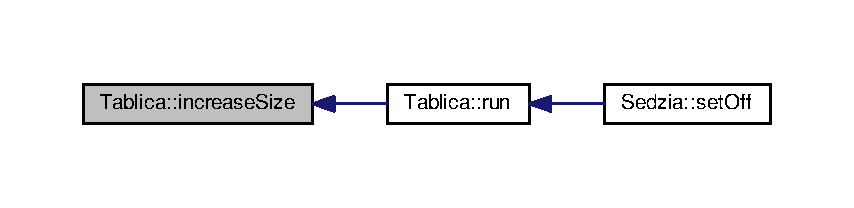
\includegraphics[width=350pt]{class_tablica_a6c8a0a055eb2bda8e7e76cc5b7690652_icgraph}
\end{center}
\end{figure}


\hypertarget{class_tablica_afbabf1c6a51051bd69c04e6c7306938c}{\index{Tablica@{Tablica}!is\-Full@{is\-Full}}
\index{is\-Full@{is\-Full}!Tablica@{Tablica}}
\subsubsection[{is\-Full}]{\setlength{\rightskip}{0pt plus 5cm}template$<$class Type$>$ bool {\bf Tablica}$<$ Type $>$\-::is\-Full (
\begin{DoxyParamCaption}
{}
\end{DoxyParamCaption}
)\hspace{0.3cm}{\ttfamily [inline]}, {\ttfamily [private]}}}\label{class_tablica_afbabf1c6a51051bd69c04e6c7306938c}


Pozwala prosto okreslic, czy nalezy przydzielic pamiec. 

Metoda prywatna. Sluzy do okreslania czy nalezy wywolac metode \hyperlink{class_tablica_a6c8a0a055eb2bda8e7e76cc5b7690652}{increase\-Size()}.

\begin{DoxyReturn}{Returns}
true Pamiec pelna. Nalezy zwiekszyc rozmiar.

false Jest jeszcze wolne miejsce. 
\end{DoxyReturn}


Here is the caller graph for this function\-:
\nopagebreak
\begin{figure}[H]
\begin{center}
\leavevmode
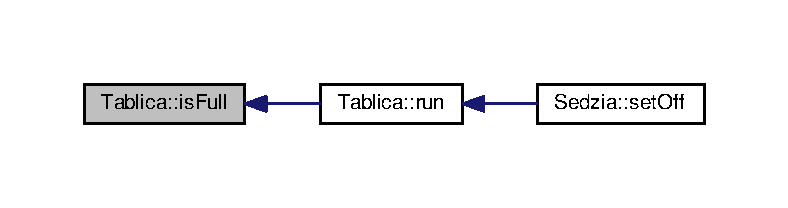
\includegraphics[width=350pt]{class_tablica_afbabf1c6a51051bd69c04e6c7306938c_icgraph}
\end{center}
\end{figure}


\hypertarget{class_tablica_ac54e8c5dcbd665dcf48d10b9df8ff41b}{\index{Tablica@{Tablica}!prepare@{prepare}}
\index{prepare@{prepare}!Tablica@{Tablica}}
\subsubsection[{prepare}]{\setlength{\rightskip}{0pt plus 5cm}template$<$class Type$>$ virtual void {\bf Tablica}$<$ Type $>$\-::prepare (
\begin{DoxyParamCaption}
\item[{{\bf uint}}]{size}
\end{DoxyParamCaption}
)\hspace{0.3cm}{\ttfamily [inline]}, {\ttfamily [virtual]}}}\label{class_tablica_ac54e8c5dcbd665dcf48d10b9df8ff41b}


Implementacja funkcji \hyperlink{class_tablica_ac54e8c5dcbd665dcf48d10b9df8ff41b}{prepare()} interfesju \hyperlink{class_i_runnable}{I\-Runnable}. 

Zapisuje pozadany rozmiar do pola desired\-\_\-size.


\begin{DoxyParams}{Parameters}
{\em size} & Parametr typu unsigned int, gdyz rozmiar nie powinien nigdy byc ujemny. Jego wartosc zapisywana jest do pola desired\-\_\-size. \\
\hline
\end{DoxyParams}


Implements \hyperlink{class_i_runnable_ac4d20dee4cb12c42eeed8698e839ddaf}{I\-Runnable}.



Here is the caller graph for this function\-:
\nopagebreak
\begin{figure}[H]
\begin{center}
\leavevmode
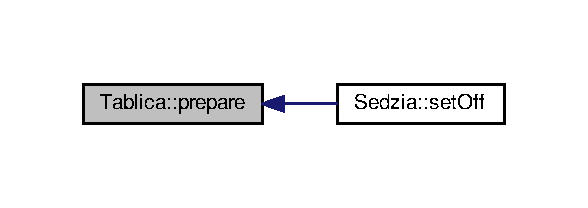
\includegraphics[width=282pt]{class_tablica_ac54e8c5dcbd665dcf48d10b9df8ff41b_icgraph}
\end{center}
\end{figure}


\hypertarget{class_tablica_a0e9570529b80cc6e1b40bf8b0d7e55c1}{\index{Tablica@{Tablica}!run@{run}}
\index{run@{run}!Tablica@{Tablica}}
\subsubsection[{run}]{\setlength{\rightskip}{0pt plus 5cm}template$<$class Type$>$ virtual void {\bf Tablica}$<$ Type $>$\-::run (
\begin{DoxyParamCaption}
{}
\end{DoxyParamCaption}
)\hspace{0.3cm}{\ttfamily [inline]}, {\ttfamily [virtual]}}}\label{class_tablica_a0e9570529b80cc6e1b40bf8b0d7e55c1}


Implementacja funkcji \hyperlink{class_tablica_a0e9570529b80cc6e1b40bf8b0d7e55c1}{run()} interfesju \hyperlink{class_i_runnable}{I\-Runnable}. 

Uruchamia \char`\"{}bieg\char`\"{}, w ktorym nastepuje zapis elementow do poszczegolnych elementow tablicy dynamicznej. Tam odbywa sie alokacja pamieci oraz instrukcje warunkowe. 

Implements \hyperlink{class_i_runnable_a6566fc2aa9fb5a7136f960172cee918d}{I\-Runnable}.



Here is the call graph for this function\-:
\nopagebreak
\begin{figure}[H]
\begin{center}
\leavevmode
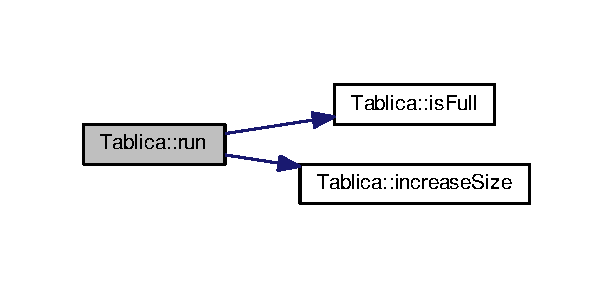
\includegraphics[width=294pt]{class_tablica_a0e9570529b80cc6e1b40bf8b0d7e55c1_cgraph}
\end{center}
\end{figure}




Here is the caller graph for this function\-:
\nopagebreak
\begin{figure}[H]
\begin{center}
\leavevmode
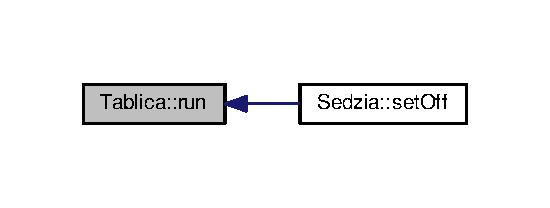
\includegraphics[width=264pt]{class_tablica_a0e9570529b80cc6e1b40bf8b0d7e55c1_icgraph}
\end{center}
\end{figure}




\subsection{Member Data Documentation}
\hypertarget{class_tablica_aa2313b2db3dfda306acaf2a28be00707}{\index{Tablica@{Tablica}!current\-\_\-size@{current\-\_\-size}}
\index{current\-\_\-size@{current\-\_\-size}!Tablica@{Tablica}}
\subsubsection[{current\-\_\-size}]{\setlength{\rightskip}{0pt plus 5cm}template$<$class Type$>$ {\bf uint} {\bf Tablica}$<$ Type $>$\-::current\-\_\-size\hspace{0.3cm}{\ttfamily [private]}}}\label{class_tablica_aa2313b2db3dfda306acaf2a28be00707}


Okresla aktualny rozmiar stosu. 

Pole prywatne typu unsigned int, gdyz rozmiar nigdy nie powinien byc ujemny. \hypertarget{class_tablica_ab9bd8738c20ec1d02ceff156af4675bc}{\index{Tablica@{Tablica}!desired\-\_\-size@{desired\-\_\-size}}
\index{desired\-\_\-size@{desired\-\_\-size}!Tablica@{Tablica}}
\subsubsection[{desired\-\_\-size}]{\setlength{\rightskip}{0pt plus 5cm}template$<$class Type$>$ {\bf uint} {\bf Tablica}$<$ Type $>$\-::desired\-\_\-size\hspace{0.3cm}{\ttfamily [private]}}}\label{class_tablica_ab9bd8738c20ec1d02ceff156af4675bc}


Okresla pozadany rozmiar stosu. 

Pole prywatne typu unsigned int, gdyz rozmiar nigdy nie powinien byc ujemny. Zadawane w funkcji \hyperlink{class_tablica_ac54e8c5dcbd665dcf48d10b9df8ff41b}{prepare()}. \hypertarget{class_tablica_a03f7862b518bdd503051388389949257}{\index{Tablica@{Tablica}!elements@{elements}}
\index{elements@{elements}!Tablica@{Tablica}}
\subsubsection[{elements}]{\setlength{\rightskip}{0pt plus 5cm}template$<$class Type$>$ Type$\ast$ {\bf Tablica}$<$ Type $>$\-::elements\hspace{0.3cm}{\ttfamily [private]}}}\label{class_tablica_a03f7862b518bdd503051388389949257}


Wskaznik do poczatku tablicy dynamicznej. 

Wskazuje na adres w pamieci sterty. Pole prywatne. \hypertarget{class_tablica_ab05112ff73217668c456d7a92273574e}{\index{Tablica@{Tablica}!index@{index}}
\index{index@{index}!Tablica@{Tablica}}
\subsubsection[{index}]{\setlength{\rightskip}{0pt plus 5cm}template$<$class Type$>$ unsigned int {\bf Tablica}$<$ Type $>$\-::index\hspace{0.3cm}{\ttfamily [private]}}}\label{class_tablica_ab05112ff73217668c456d7a92273574e}


Okresla aktualny indeks. 

Pole prywatne typu unsigned int, gdyz indeks nigdy nie powinien byc ujemny. Przechowuje indeks, pierwszej wolnej komorki pamieci, do ktorego mozliwy bedzie zapis. 

The documentation for this class was generated from the following file\-:\begin{DoxyCompactItemize}
\item 
inc/\hyperlink{_tablica_8h}{Tablica.\-h}\end{DoxyCompactItemize}

\chapter{File Documentation}
\hypertarget{_i_lista_8h}{\section{inc/\-I\-Lista.h File Reference}
\label{_i_lista_8h}\index{inc/\-I\-Lista.\-h@{inc/\-I\-Lista.\-h}}
}


Plik zawiera interfejs dla pojemnika \hyperlink{class_lista}{Lista} oraz dla klasy Wezel.  


{\ttfamily \#include $<$cstddef$>$}\\*
Include dependency graph for I\-Lista.\-h\-:
\nopagebreak
\begin{figure}[H]
\begin{center}
\leavevmode
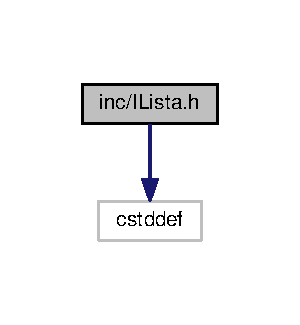
\includegraphics[width=144pt]{_i_lista_8h__incl}
\end{center}
\end{figure}
This graph shows which files directly or indirectly include this file\-:
\nopagebreak
\begin{figure}[H]
\begin{center}
\leavevmode
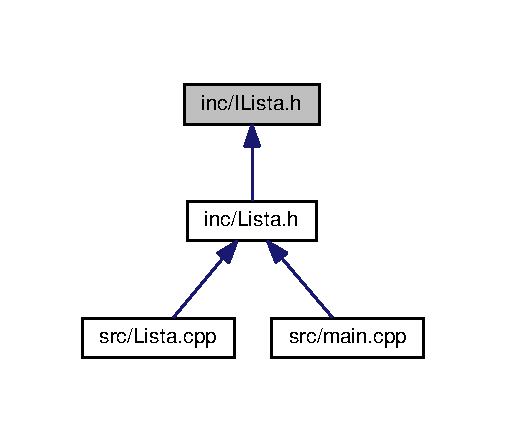
\includegraphics[width=243pt]{_i_lista_8h__dep__incl}
\end{center}
\end{figure}
\subsection*{Classes}
\begin{DoxyCompactItemize}
\item 
class \hyperlink{class_node}{Node$<$ Node\-Type $>$}
\begin{DoxyCompactList}\small\item\em Imlementacja wezlow dla listy. \end{DoxyCompactList}\item 
class \hyperlink{class_i_lista}{I\-Lista$<$ List\-Type $>$}
\begin{DoxyCompactList}\small\item\em Interfejs dla pojemnika \hyperlink{class_lista}{Lista}. \end{DoxyCompactList}\end{DoxyCompactItemize}
\subsection*{Typedefs}
\begin{DoxyCompactItemize}
\item 
typedef unsigned int \hyperlink{_i_lista_8h_a91ad9478d81a7aaf2593e8d9c3d06a14}{uint}
\begin{DoxyCompactList}\small\item\em Skraca zapis. \end{DoxyCompactList}\end{DoxyCompactItemize}


\subsection{Detailed Description}
Plik zawiera interfejs dla pojemnika \hyperlink{class_lista}{Lista} oraz dla klasy Wezel. Wskutek zastosowania szablonow wszystkie definicje musza znajdowac sie w pliku naglowkowym, a nie zrodlowym. Wezel jest elementem listy.

\begin{DoxyAuthor}{Author}
Kamil Kuczaj. 
\end{DoxyAuthor}


\subsection{Typedef Documentation}
\hypertarget{_i_lista_8h_a91ad9478d81a7aaf2593e8d9c3d06a14}{\index{I\-Lista.\-h@{I\-Lista.\-h}!uint@{uint}}
\index{uint@{uint}!ILista.h@{I\-Lista.\-h}}
\subsubsection[{uint}]{\setlength{\rightskip}{0pt plus 5cm}typedef unsigned int {\bf uint}}}\label{_i_lista_8h_a91ad9478d81a7aaf2593e8d9c3d06a14}


Skraca zapis. 

Zdefiniowanie wlasnego typu -\/ pozwala na krotszy zapis. 
\hypertarget{_i_pojemnik_8h}{\section{inc/\-I\-Pojemnik.h File Reference}
\label{_i_pojemnik_8h}\index{inc/\-I\-Pojemnik.\-h@{inc/\-I\-Pojemnik.\-h}}
}


Plik zawiera interfejs dla pojemnika Stos, \hyperlink{class_kolejka}{Kolejka} oraz \hyperlink{class_tablica}{Tablica}.  


This graph shows which files directly or indirectly include this file\-:
\nopagebreak
\begin{figure}[H]
\begin{center}
\leavevmode
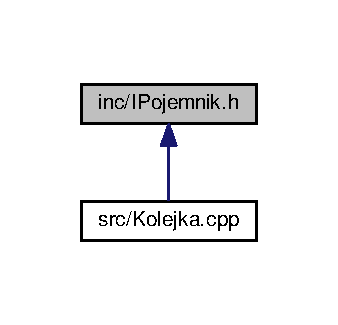
\includegraphics[width=162pt]{_i_pojemnik_8h__dep__incl}
\end{center}
\end{figure}
\subsection*{Classes}
\begin{DoxyCompactItemize}
\item 
class \hyperlink{class_i_pojemnik}{I\-Pojemnik$<$ Type $>$}
\begin{DoxyCompactList}\small\item\em Interfejs dla każdego pojemnika. \end{DoxyCompactList}\end{DoxyCompactItemize}
\subsection*{Typedefs}
\begin{DoxyCompactItemize}
\item 
typedef unsigned int \hyperlink{_i_pojemnik_8h_a91ad9478d81a7aaf2593e8d9c3d06a14}{uint}
\begin{DoxyCompactList}\small\item\em Skraca zapis. \end{DoxyCompactList}\end{DoxyCompactItemize}


\subsection{Detailed Description}
Plik zawiera interfejs dla pojemnika Stos, \hyperlink{class_kolejka}{Kolejka} oraz \hyperlink{class_tablica}{Tablica}. Wskutek zastosowania szablonow wszystkie definicje musza znajdowac sie w pliku naglowkowym, a nie zrodlowym.

\begin{DoxyAuthor}{Author}
Kamil Kuczaj. 
\end{DoxyAuthor}


\subsection{Typedef Documentation}
\hypertarget{_i_pojemnik_8h_a91ad9478d81a7aaf2593e8d9c3d06a14}{\index{I\-Pojemnik.\-h@{I\-Pojemnik.\-h}!uint@{uint}}
\index{uint@{uint}!IPojemnik.h@{I\-Pojemnik.\-h}}
\subsubsection[{uint}]{\setlength{\rightskip}{0pt plus 5cm}typedef unsigned int {\bf uint}}}\label{_i_pojemnik_8h_a91ad9478d81a7aaf2593e8d9c3d06a14}


Skraca zapis. 

Zdefiniowanie wlasnego typu -\/ pozwala na krotszy zapis. 
\hypertarget{_i_runnable_8h}{\section{inc/\-I\-Runnable.h File Reference}
\label{_i_runnable_8h}\index{inc/\-I\-Runnable.\-h@{inc/\-I\-Runnable.\-h}}
}


Naglowek zawierajacy interfejs dla biegacza.  


This graph shows which files directly or indirectly include this file\-:
\nopagebreak
\begin{figure}[H]
\begin{center}
\leavevmode
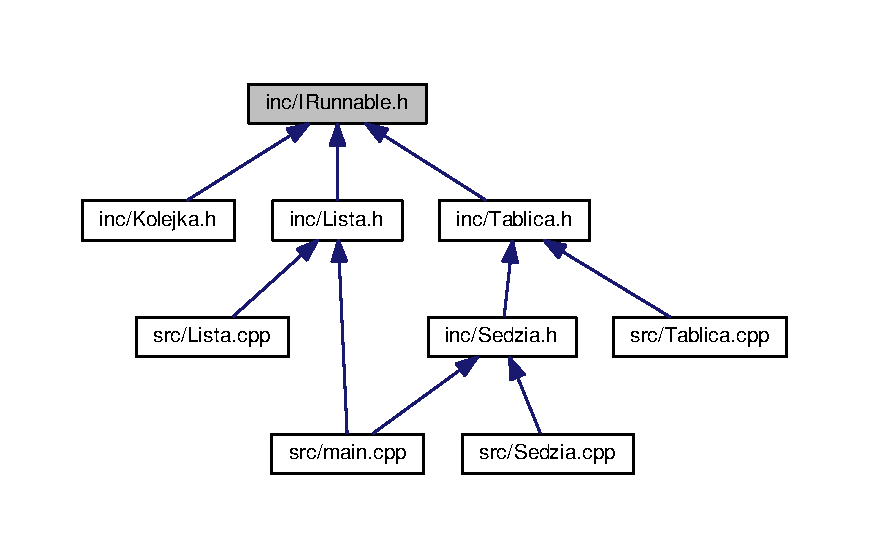
\includegraphics[width=350pt]{_i_runnable_8h__dep__incl}
\end{center}
\end{figure}
\subsection*{Classes}
\begin{DoxyCompactItemize}
\item 
class \hyperlink{class_i_runnable}{I\-Runnable}
\begin{DoxyCompactList}\small\item\em Interfejs dla biegacza. \end{DoxyCompactList}\end{DoxyCompactItemize}


\subsection{Detailed Description}
Naglowek zawierajacy interfejs dla biegacza. \begin{DoxyAuthor}{Author}
Kamil Kuczaj 
\end{DoxyAuthor}

\hypertarget{_i_stoper_8h}{\section{inc/\-I\-Stoper.h File Reference}
\label{_i_stoper_8h}\index{inc/\-I\-Stoper.\-h@{inc/\-I\-Stoper.\-h}}
}


Naglowek zawierajacy interfejs dla stopera.  


{\ttfamily \#include $<$string$>$}\\*
Include dependency graph for I\-Stoper.\-h\-:
\nopagebreak
\begin{figure}[H]
\begin{center}
\leavevmode
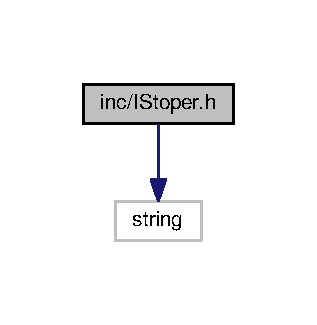
\includegraphics[width=152pt]{_i_stoper_8h__incl}
\end{center}
\end{figure}
This graph shows which files directly or indirectly include this file\-:
\nopagebreak
\begin{figure}[H]
\begin{center}
\leavevmode
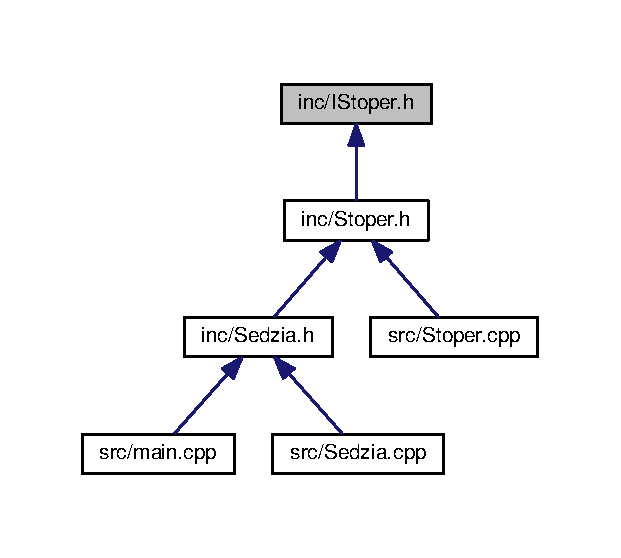
\includegraphics[width=298pt]{_i_stoper_8h__dep__incl}
\end{center}
\end{figure}
\subsection*{Classes}
\begin{DoxyCompactItemize}
\item 
class \hyperlink{class_i_stoper}{I\-Stoper}
\begin{DoxyCompactList}\small\item\em Interfejs dla stopera. \end{DoxyCompactList}\end{DoxyCompactItemize}


\subsection{Detailed Description}
Naglowek zawierajacy interfejs dla stopera. \begin{DoxyAuthor}{Author}
Kamil Kuczaj 
\end{DoxyAuthor}

\hypertarget{_kolejka_8h}{\section{inc/\-Kolejka.h File Reference}
\label{_kolejka_8h}\index{inc/\-Kolejka.\-h@{inc/\-Kolejka.\-h}}
}
{\ttfamily \#include \char`\"{}I\-Runnable.\-h\char`\"{}}\\*
Include dependency graph for Kolejka.\-h\-:
\nopagebreak
\begin{figure}[H]
\begin{center}
\leavevmode
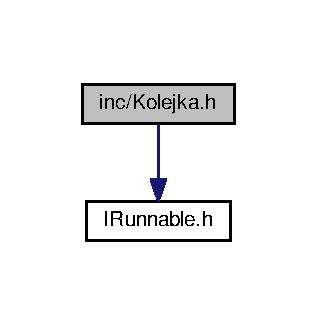
\includegraphics[width=152pt]{_kolejka_8h__incl}
\end{center}
\end{figure}
\subsection*{Classes}
\begin{DoxyCompactItemize}
\item 
class \hyperlink{class_kolejka}{Kolejka}
\end{DoxyCompactItemize}

\hypertarget{_lista_8h}{\section{inc/\-Lista.h File Reference}
\label{_lista_8h}\index{inc/\-Lista.\-h@{inc/\-Lista.\-h}}
}


Implementacja jednokierunkowej listy.  


{\ttfamily \#include \char`\"{}I\-Runnable.\-h\char`\"{}}\\*
{\ttfamily \#include \char`\"{}I\-Lista.\-h\char`\"{}}\\*
{\ttfamily \#include $<$cstddef$>$}\\*
{\ttfamily \#include $<$string$>$}\\*
{\ttfamily \#include $<$iostream$>$}\\*
{\ttfamily \#include $<$fstream$>$}\\*
Include dependency graph for Lista.\-h\-:
\nopagebreak
\begin{figure}[H]
\begin{center}
\leavevmode
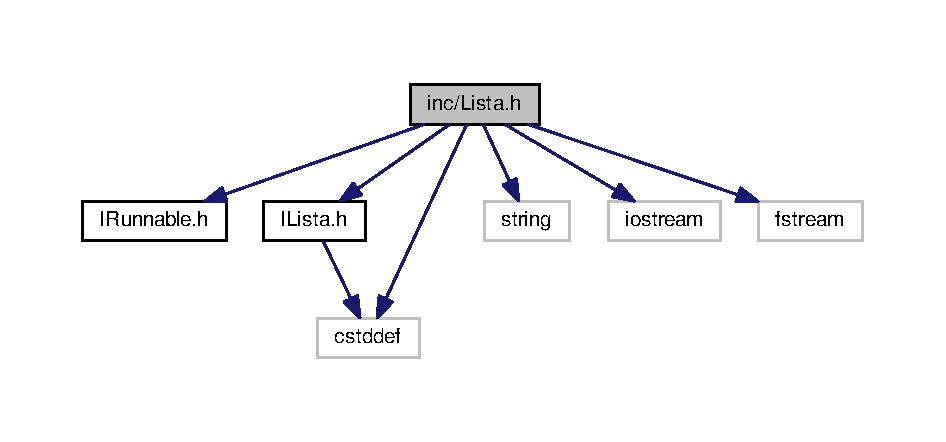
\includegraphics[width=350pt]{_lista_8h__incl}
\end{center}
\end{figure}
This graph shows which files directly or indirectly include this file\-:
\nopagebreak
\begin{figure}[H]
\begin{center}
\leavevmode
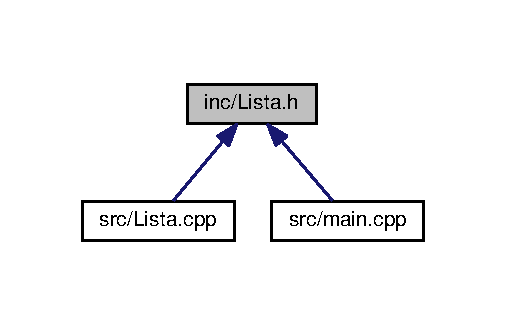
\includegraphics[width=243pt]{_lista_8h__dep__incl}
\end{center}
\end{figure}
\subsection*{Classes}
\begin{DoxyCompactItemize}
\item 
class \hyperlink{class_lista}{Lista$<$ Type $>$}
\begin{DoxyCompactList}\small\item\em Klasa \hyperlink{class_lista}{Lista}, w ktorej odbywa sie zapis dynamiczny elementow typu int. \end{DoxyCompactList}\end{DoxyCompactItemize}
\subsection*{Typedefs}
\begin{DoxyCompactItemize}
\item 
typedef unsigned int \hyperlink{_lista_8h_a91ad9478d81a7aaf2593e8d9c3d06a14}{uint}
\begin{DoxyCompactList}\small\item\em Skraca zapis. \end{DoxyCompactList}\end{DoxyCompactItemize}


\subsection{Detailed Description}
Implementacja jednokierunkowej listy. Wskutek zastosowania szablonow wszystkie definicje musza znajdowac sie w pliku naglowkowym, a nie zrodlowym.

\begin{DoxyAuthor}{Author}
Kamil Kuczaj. 
\end{DoxyAuthor}


\subsection{Typedef Documentation}
\hypertarget{_lista_8h_a91ad9478d81a7aaf2593e8d9c3d06a14}{\index{Lista.\-h@{Lista.\-h}!uint@{uint}}
\index{uint@{uint}!Lista.h@{Lista.\-h}}
\subsubsection[{uint}]{\setlength{\rightskip}{0pt plus 5cm}typedef unsigned int {\bf uint}}}\label{_lista_8h_a91ad9478d81a7aaf2593e8d9c3d06a14}


Skraca zapis. 

Zdefiniowanie wlasnego typu -\/ pozwala na krotszy zapis 
\hypertarget{_sedzia_8h}{\section{inc/\-Sedzia.h File Reference}
\label{_sedzia_8h}\index{inc/\-Sedzia.\-h@{inc/\-Sedzia.\-h}}
}


Naglowek opisujacy implementacje Sedziego.  


{\ttfamily \#include \char`\"{}Stoper.\-h\char`\"{}}\\*
{\ttfamily \#include \char`\"{}Tablica.\-h\char`\"{}}\\*
{\ttfamily \#include $<$iostream$>$}\\*
{\ttfamily \#include $<$iomanip$>$}\\*
{\ttfamily \#include $<$sstream$>$}\\*
Include dependency graph for Sedzia.\-h\-:
\nopagebreak
\begin{figure}[H]
\begin{center}
\leavevmode
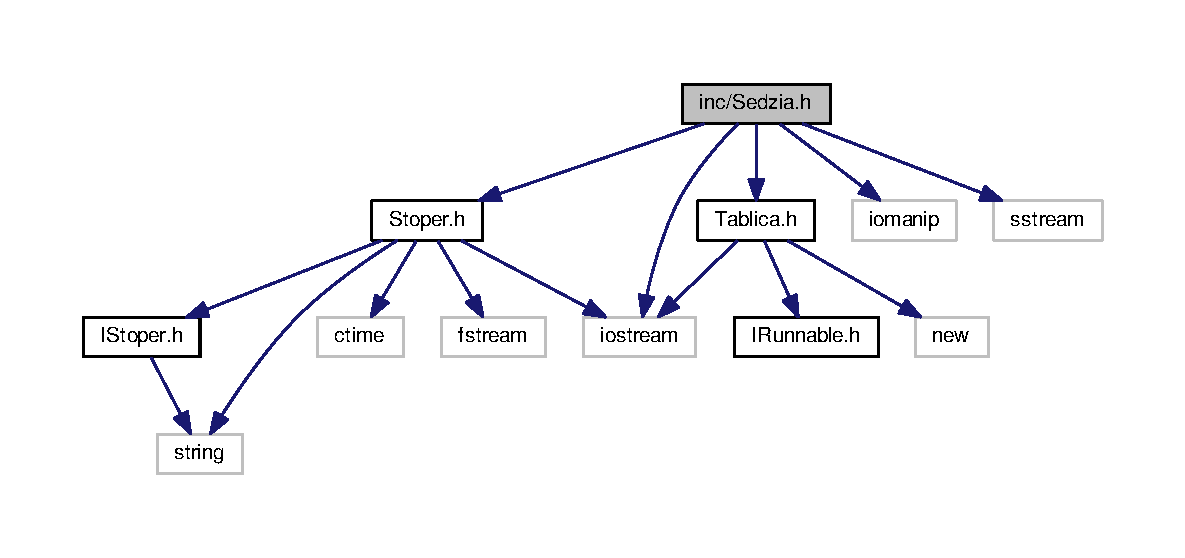
\includegraphics[width=350pt]{_sedzia_8h__incl}
\end{center}
\end{figure}
This graph shows which files directly or indirectly include this file\-:
\nopagebreak
\begin{figure}[H]
\begin{center}
\leavevmode
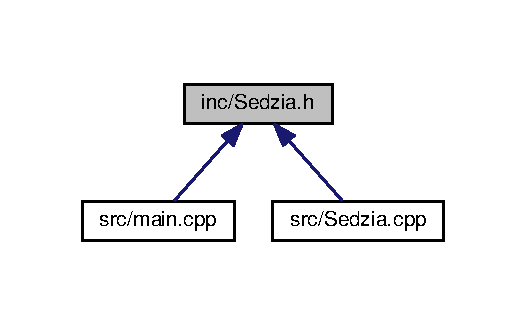
\includegraphics[width=253pt]{_sedzia_8h__dep__incl}
\end{center}
\end{figure}
\subsection*{Classes}
\begin{DoxyCompactItemize}
\item 
class \hyperlink{class_sedzia}{Sedzia}
\begin{DoxyCompactList}\small\item\em Implementacja klasy \hyperlink{class_sedzia}{Sedzia}. \end{DoxyCompactList}\end{DoxyCompactItemize}


\subsection{Detailed Description}
Naglowek opisujacy implementacje Sedziego. \begin{DoxyAuthor}{Author}
Kamil Kuczaj 
\end{DoxyAuthor}

\hypertarget{_stoper_8h}{\section{inc/\-Stoper.h File Reference}
\label{_stoper_8h}\index{inc/\-Stoper.\-h@{inc/\-Stoper.\-h}}
}


Implementacja interfejsu \hyperlink{class_i_stoper}{I\-Stoper} w klasie \hyperlink{class_stoper}{Stoper}.  


{\ttfamily \#include \char`\"{}I\-Stoper.\-h\char`\"{}}\\*
{\ttfamily \#include $<$ctime$>$}\\*
{\ttfamily \#include $<$fstream$>$}\\*
{\ttfamily \#include $<$iostream$>$}\\*
{\ttfamily \#include $<$string$>$}\\*
Include dependency graph for Stoper.\-h\-:
\nopagebreak
\begin{figure}[H]
\begin{center}
\leavevmode
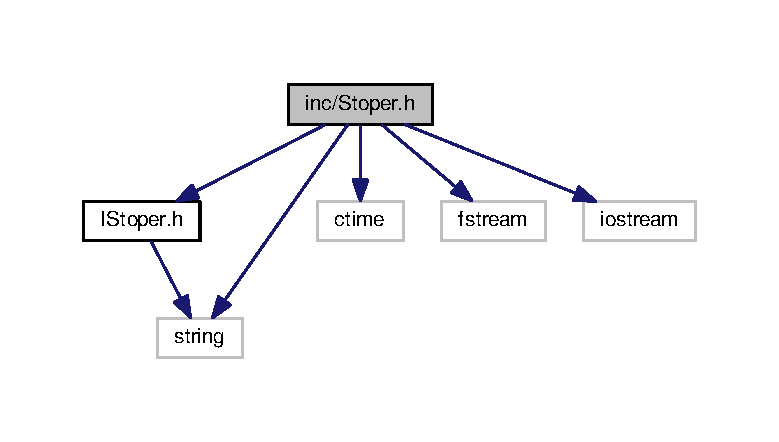
\includegraphics[width=350pt]{_stoper_8h__incl}
\end{center}
\end{figure}
This graph shows which files directly or indirectly include this file\-:
\nopagebreak
\begin{figure}[H]
\begin{center}
\leavevmode
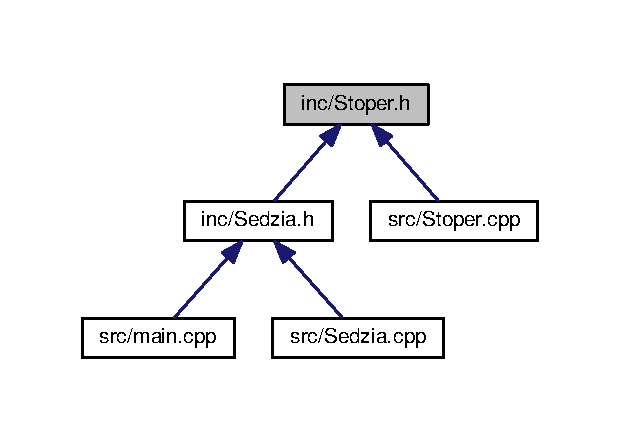
\includegraphics[width=298pt]{_stoper_8h__dep__incl}
\end{center}
\end{figure}
\subsection*{Classes}
\begin{DoxyCompactItemize}
\item 
class \hyperlink{class_stoper}{Stoper}
\begin{DoxyCompactList}\small\item\em Implementacja klasy \hyperlink{class_stoper}{Stoper}. \end{DoxyCompactList}\end{DoxyCompactItemize}


\subsection{Detailed Description}
Implementacja interfejsu \hyperlink{class_i_stoper}{I\-Stoper} w klasie \hyperlink{class_stoper}{Stoper}. \begin{DoxyAuthor}{Author}
Kamil Kuczaj 
\end{DoxyAuthor}

\hypertarget{_stos_8h}{\section{inc/\-Stos.h File Reference}
\label{_stos_8h}\index{inc/\-Stos.\-h@{inc/\-Stos.\-h}}
}

\hypertarget{_tablica_8h}{\section{inc/\-Tablica.h File Reference}
\label{_tablica_8h}\index{inc/\-Tablica.\-h@{inc/\-Tablica.\-h}}
}


Implementacja interfesju \hyperlink{class_i_runnable}{I\-Runnable}.  


{\ttfamily \#include \char`\"{}I\-Runnable.\-h\char`\"{}}\\*
{\ttfamily \#include $<$new$>$}\\*
{\ttfamily \#include $<$iostream$>$}\\*
Include dependency graph for Tablica.\-h\-:
\nopagebreak
\begin{figure}[H]
\begin{center}
\leavevmode
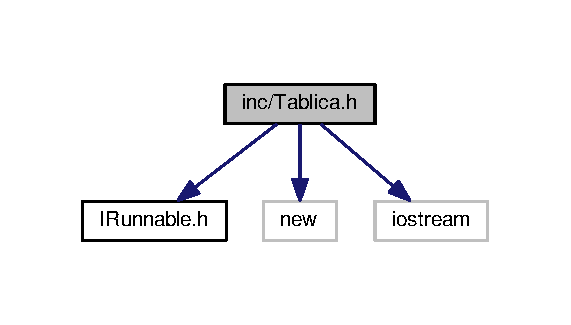
\includegraphics[width=274pt]{_tablica_8h__incl}
\end{center}
\end{figure}
This graph shows which files directly or indirectly include this file\-:
\nopagebreak
\begin{figure}[H]
\begin{center}
\leavevmode
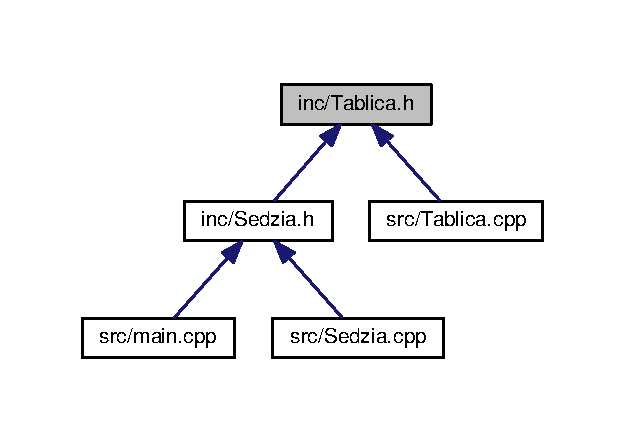
\includegraphics[width=300pt]{_tablica_8h__dep__incl}
\end{center}
\end{figure}
\subsection*{Classes}
\begin{DoxyCompactItemize}
\item 
class \hyperlink{class_tablica}{Tablica$<$ Type $>$}
\begin{DoxyCompactList}\small\item\em Klasa \hyperlink{class_tablica}{Tablica}, w ktorej odbywa sie zapis dynamiczny elementow. \end{DoxyCompactList}\end{DoxyCompactItemize}
\subsection*{Typedefs}
\begin{DoxyCompactItemize}
\item 
typedef unsigned int \hyperlink{_tablica_8h_a91ad9478d81a7aaf2593e8d9c3d06a14}{uint}
\begin{DoxyCompactList}\small\item\em Skraca zapis. \end{DoxyCompactList}\end{DoxyCompactItemize}


\subsection{Detailed Description}
Implementacja interfesju \hyperlink{class_i_runnable}{I\-Runnable}. \begin{DoxyAuthor}{Author}
Kamil Kuczaj 
\end{DoxyAuthor}


\subsection{Typedef Documentation}
\hypertarget{_tablica_8h_a91ad9478d81a7aaf2593e8d9c3d06a14}{\index{Tablica.\-h@{Tablica.\-h}!uint@{uint}}
\index{uint@{uint}!Tablica.h@{Tablica.\-h}}
\subsubsection[{uint}]{\setlength{\rightskip}{0pt plus 5cm}typedef unsigned int {\bf uint}}}\label{_tablica_8h_a91ad9478d81a7aaf2593e8d9c3d06a14}


Skraca zapis. 

Zdefiniowanie wlasnego typu -\/ pozwala na krotszy zapis 
\hypertarget{_kolejka_8cpp}{\section{src/\-Kolejka.cpp File Reference}
\label{_kolejka_8cpp}\index{src/\-Kolejka.\-cpp@{src/\-Kolejka.\-cpp}}
}
{\ttfamily \#include \char`\"{}I\-Pojemnik.\-h\char`\"{}}\\*
Include dependency graph for Kolejka.\-cpp\-:
\nopagebreak
\begin{figure}[H]
\begin{center}
\leavevmode
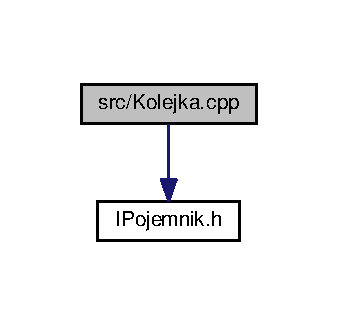
\includegraphics[width=162pt]{_kolejka_8cpp__incl}
\end{center}
\end{figure}

\hypertarget{_lista_8cpp}{\section{src/\-Lista.cpp File Reference}
\label{_lista_8cpp}\index{src/\-Lista.\-cpp@{src/\-Lista.\-cpp}}
}
{\ttfamily \#include \char`\"{}Lista.\-h\char`\"{}}\\*
Include dependency graph for Lista.\-cpp\-:
\nopagebreak
\begin{figure}[H]
\begin{center}
\leavevmode
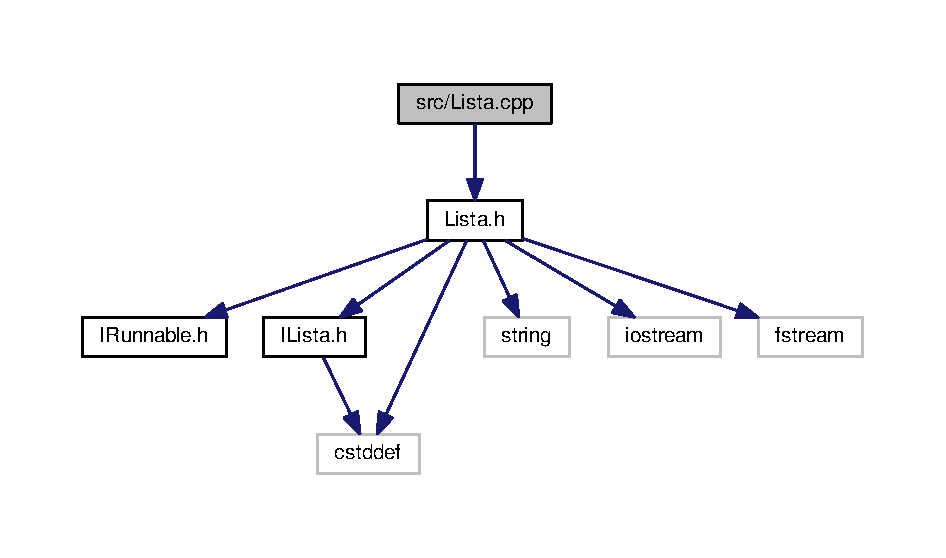
\includegraphics[width=350pt]{_lista_8cpp__incl}
\end{center}
\end{figure}

\hypertarget{main_8cpp}{\section{src/main.cpp File Reference}
\label{main_8cpp}\index{src/main.\-cpp@{src/main.\-cpp}}
}
{\ttfamily \#include \char`\"{}Sedzia.\-h\char`\"{}}\\*
{\ttfamily \#include \char`\"{}Lista.\-h\char`\"{}}\\*
{\ttfamily \#include $<$iostream$>$}\\*
{\ttfamily \#include $<$ctime$>$}\\*
{\ttfamily \#include $<$iomanip$>$}\\*
{\ttfamily \#include $<$string$>$}\\*
Include dependency graph for main.\-cpp\-:
\nopagebreak
\begin{figure}[H]
\begin{center}
\leavevmode
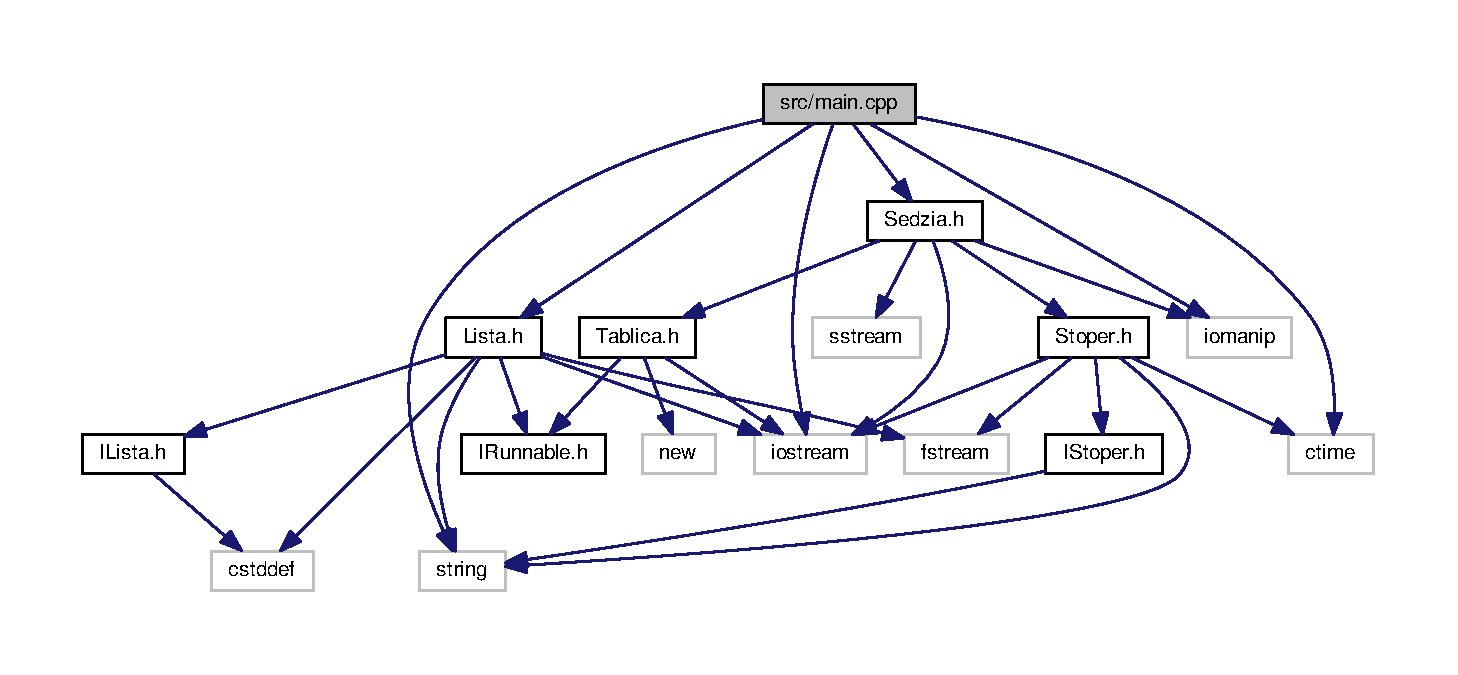
\includegraphics[width=350pt]{main_8cpp__incl}
\end{center}
\end{figure}
\subsection*{Functions}
\begin{DoxyCompactItemize}
\item 
int \hyperlink{main_8cpp_a3c04138a5bfe5d72780bb7e82a18e627}{main} (int argc, char $\ast$$\ast$argv)
\end{DoxyCompactItemize}


\subsection{Function Documentation}
\hypertarget{main_8cpp_a3c04138a5bfe5d72780bb7e82a18e627}{\index{main.\-cpp@{main.\-cpp}!main@{main}}
\index{main@{main}!main.cpp@{main.\-cpp}}
\subsubsection[{main}]{\setlength{\rightskip}{0pt plus 5cm}int main (
\begin{DoxyParamCaption}
\item[{int}]{argc, }
\item[{char $\ast$$\ast$}]{argv}
\end{DoxyParamCaption}
)}}\label{main_8cpp_a3c04138a5bfe5d72780bb7e82a18e627}


Here is the call graph for this function\-:
\nopagebreak
\begin{figure}[H]
\begin{center}
\leavevmode
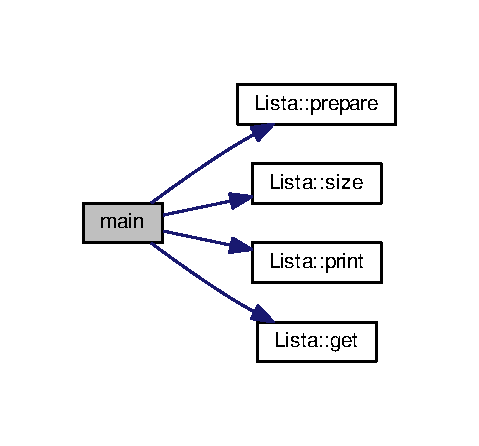
\includegraphics[width=230pt]{main_8cpp_a3c04138a5bfe5d72780bb7e82a18e627_cgraph}
\end{center}
\end{figure}



\hypertarget{_sedzia_8cpp}{\section{src/\-Sedzia.cpp File Reference}
\label{_sedzia_8cpp}\index{src/\-Sedzia.\-cpp@{src/\-Sedzia.\-cpp}}
}
{\ttfamily \#include \char`\"{}Sedzia.\-h\char`\"{}}\\*
Include dependency graph for Sedzia.\-cpp\-:
\nopagebreak
\begin{figure}[H]
\begin{center}
\leavevmode
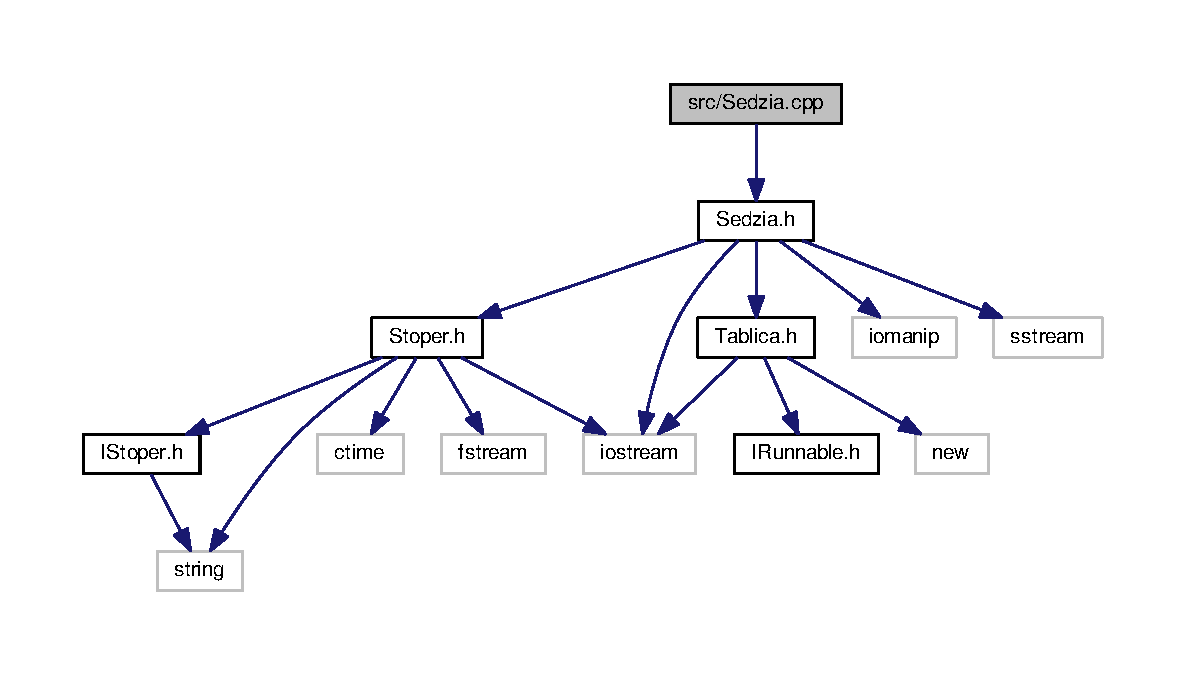
\includegraphics[width=350pt]{_sedzia_8cpp__incl}
\end{center}
\end{figure}

\hypertarget{_stoper_8cpp}{\section{src/\-Stoper.cpp File Reference}
\label{_stoper_8cpp}\index{src/\-Stoper.\-cpp@{src/\-Stoper.\-cpp}}
}
{\ttfamily \#include \char`\"{}Stoper.\-h\char`\"{}}\\*
Include dependency graph for Stoper.\-cpp\-:
\nopagebreak
\begin{figure}[H]
\begin{center}
\leavevmode
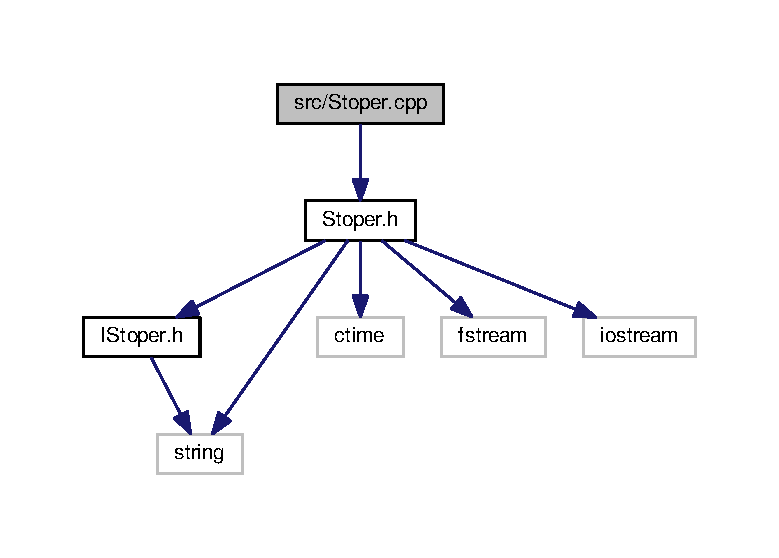
\includegraphics[width=350pt]{_stoper_8cpp__incl}
\end{center}
\end{figure}

\hypertarget{_stos_8cpp}{\section{src/\-Stos.cpp File Reference}
\label{_stos_8cpp}\index{src/\-Stos.\-cpp@{src/\-Stos.\-cpp}}
}

\hypertarget{_tablica_8cpp}{\section{src/\-Tablica.cpp File Reference}
\label{_tablica_8cpp}\index{src/\-Tablica.\-cpp@{src/\-Tablica.\-cpp}}
}
{\ttfamily \#include \char`\"{}Tablica.\-h\char`\"{}}\\*
Include dependency graph for Tablica.\-cpp\-:
\nopagebreak
\begin{figure}[H]
\begin{center}
\leavevmode
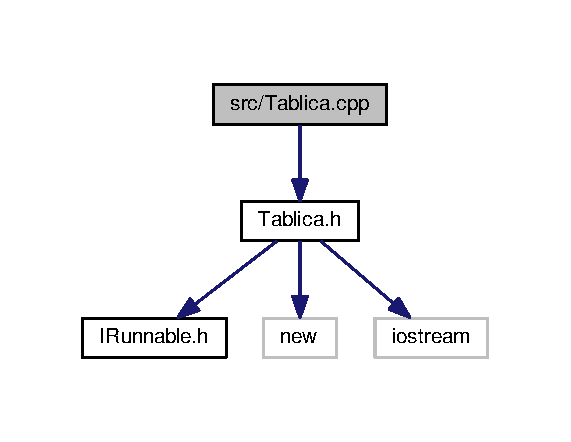
\includegraphics[width=274pt]{_tablica_8cpp__incl}
\end{center}
\end{figure}

%--- End generated contents ---

% Index
\newpage
\phantomsection
\addcontentsline{toc}{chapter}{Index}
\printindex

\end{document}
